\uselanguage{French}
\languagepath{French}

\usepackage[utf8]{inputenc}
\usepackage[T1]{fontenc}
\usepackage{lmodern}
\usepackage{amssymb,amsmath,amsthm}
\usepackage{textcomp}
\usepackage{graphics}
\usepackage[absolute,overlay]{textpos}
\usepackage{fancyvrb}
\usepackage{tikz}
\usepackage{colortbl}
\usepackage{array}
\usepackage{hhline}
\usepackage{xspace}
\usepackage{bclogo}
\usepackage{makecell}
\usepackage{multicol}
\usepackage{style-esi/licence}
\usepackage{style-esi/links}
% import commands and styles used in the syllabus.
\usepackage{dev1/cours-developpement/syllabus/styles/esi-flowchart}
\usepackage{dev1/cours-developpement/syllabus/styles/flow}
\usepackage{dev1/cours-developpement/syllabus/styles/java}
\usepackage{dev1/cours-developpement/syllabus/styles/terminal}
\usepackage{dev1/cours-developpement/syllabus/styles/langagenaturel}
\usepackage{dev1/cours-developpement/syllabus/styles/pseudocode}
\usepackage{comment}

\newcommand*{\sybprffx}{dev1/cours-developpement/syllabus}

\newenvironment{wrong}[1][<1>]{%
  \begin{minipage}{\linewidth}}
  {\end{minipage}
  \pause
  \hskip-5em
  \raisebox{-1em}{
    \includegraphics[width=4em]{\sybprffx/icon/dont}}
}

% cf. Syllabus MAT1.
\newcommand{\xor}{ \raisebox{-0.05cm}{ %ole %do not use index or in tikzpicture
\begin{tikzpicture}[scale=0.175]
\draw (120:1) -- (0,0) -- (60:1);
\draw (-0.6,-0.35) -- (0.6,-0.35);
\end{tikzpicture}
} }

% The default decision block was too big.
\tikzstyle{decision} = [
  diamond,
  minimum width=2cm,
  minimum height=1cm,
  text centered,
  text width=2cm,
  draw=black,
  fill=green!30]

\tikzset{
  connector/.style={
   -latex,
   font=\scriptsize
  },
  rectangle connector/.style={
    connector,
    to path={(\tikztostart) -- ++(#1,0pt) \tikztonodes |- (\tikztotarget) },
    pos=0.5
  },
  rectangle connector/.default=-2cm,
  straight connector/.style={
    connector,
    to path=--(\tikztotarget) \tikztonodes
  }
}

\newenvironment<>{varblock}[2][\textwidth]{%
  \setlength{\textwidth}{#1}%
  \begin{actionenv}#3%
  \def\insertblocktitle{#2}%
  \par%
  \usebeamertemplate{block begin}%
}{%
  \par%
  \usebeamertemplate{block end}%
  \end{actionenv}%
}

\renewcommand{\pc}{\texttt}

% Define \tableonly, for a \only on tables rows.
% https://tex.stackexchange.com/a/474748
\makeatletter
\newcommand*\tableonly%>>>
  {%
    \omit\@ifnextchar<\table@only\table@@only
  }%<<<
\protected\long\def\table@only<#1>#2%>>>
  {%
    \gdef\beamer@doifnotinframe{\cr}%
    \def\beamer@doifinframe{\cr#2}%
    \beamer@masterdecode{#1}%
    \beamer@donow
  }%<<<
\protected\long\def\table@@only#1%>>>
  {%
    \beamer@ifnextcharospec{\table@@@only{#1}}{\cr#1}%
  }%<<<
\long\def\table@@@only#1<#2>%>>>
  {%
    \gdef\beamer@doifnotinframe{\cr}%
    \def\beamer@doifinframe{\cr#1}%
    \beamer@masterdecode{#2}%
    \beamer@donow
  }%<<<
\makeatother

\newcommand{\developmentsteps}{
  {\sffamily
  \begin{tikzpicture}
    \matrix [row sep = 2em] {
     \node[draw, rounded corners, thick] (P1) {Analyse}; \\
     \node[draw, rounded corners, thick] (P2) {Algorithmes}; \\
     \node[draw, rounded corners, thick] (P3) {Programmation}; \\
     \node[draw, rounded corners, thick] (P4) {Tests}; \\
     \node[draw, rounded corners, thick] (P5) {Livraison}; \\
    };
    \draw[->, thick] (P1) to (P2);
    \draw[->, thick] (P2) to (P3);
    \draw[->, thick] (P3) to (P4);
    \draw[->, thick] (P4) to (P5);
  \end{tikzpicture}
}}

% Customize the section page a bit.
\setbeamertemplate{section page}{
  \medskip
  \colbox[dark,fuzzy]{\Huge\insertsectionnumber}~
  \colbox[dark,fuzzy]{
    \begin{minipage}[t]{0.5\textwidth}
      \Large\insertsection
    \end{minipage}
  }
  \hfill \raisebox{-4cm}{\developmentsteps}
}

% Enumerate continuation
\newcounter{saveenumi}
\newcommand{\seti}{\setcounter{saveenumi}{\value{enumi}}}
\newcommand{\conti}{\setcounter{enumi}{\value{saveenumi}}}

\resetcounteronoverlays{saveenumi}

% The colors defined in style-esi/links are invisible on the output beamer.
\hypersetup{colorlinks=false}

\title[DEV1-dev]{DEV1}
\subtitle{Développement}
\author[P. Hauweele (PHA)]{Pierre \textsc{Hauweele}}
\date[2020--2021]{Année académique 2020--2021}

\begin{document}
\begin{frame}[plain]
  \titlepage
\end{frame}

%\begin{frame}[plain]
%  \colbox[center,dark,lifted][center]{\LARGE Plan du cours}
%  \tableofcontents
%\end{frame}

\begin{frame}
  Ces slides sont une quasi-copie du Syllabus de développement, disponible sur
  la page du cours de DEV1 sur \href{https://poesi.esi-bru.be}{poési}.

  Ils sont écrits au fur et à mesure des séances et sont incomplets. Le
  syllabus est la référence.

  Le repository git est publique :\\
  \url{https://github.com/antegallya/dev1-slides-pha}

  Les exemples de code faits aux cours (et plus) sont publiés dans le
  sous-répertoire \href{https://github.com/antegallya/dev1-slides-pha/tree/master/exemples}
  {\texttt{exemples/}}.

  \ccbysa{phauweele@he2b.be}
\end{frame}
\begin{hideedit}

\part{Introduction}
\frame{\partpage}
\section{Résoudre des problèmes}
\frame{\sectionpage}
\section{Les algorithmes et les programmes}
\frame{\sectionpage}
\begin{frame}
  \begin{definition}[Algorithme]
    Procédure de résolution d’un problème
    contenant des opérations bien définies
    portant sur des informations,
    s’exprimant dans une séquence définie sans ambigüité,
    destinée à être traduite dans un langage de programmation.
  \end{definition}
  \begin{definition}[Programme]
    Un \textbf{programme} n’est rien d’autre
    que la représentation d’un algorithme
    dans un langage plus technique compris par un ordinateur
    (par exemple~:~Assembleur, Cobol, Java, C++\dots).
    Ce type de langage est appelé
    \textbf{langage de programmation}.
  \end{definition}
\end{frame}

\part{Bases de l'algorithmique et de la programmation}
\frame{\partpage}

\section{Spécifier le problème}
\frame{\sectionpage}
\begin{frame}{Données et résultat}
  \begin{block}{}
  \begin{center}
    {\textbf{étant donné} [les données]
    \textbf{on demande} [résultat]}
  \end{center}
  \end{block}
  \pause
  \begin{example}
    Soit l’énoncé suivant~:
    \og
      Calculer la surface d’un rectangle
      à partir de sa longueur et sa largeur
    \fg.

    Quelles sont les données~? \pause Il y en a deux~:
    \begin{itemize}
            \item la longueur du rectangle~;
            \item sa largeur.
    \end{itemize}

    \pause
    Quel est le résultat attendu~? \pause la surface du rectangle.
  \end{example}
\end{frame}

\subsection{Les noms}
\begin{frame}{Identifier les données}

  \begin{example}
  Quel nom choisir pour la longueur d’un rectangle~?

  \pause
  \begin{itemize}
    \item
      \pc{length} \pause: OK.
    \pause
    \item
      \pc{longueur} \pause: on préfère en anglais
    \pause
    \item
      \pc{rectangleLength} \pause: pour éviter toute ambigüité avec une
      autre longueur.
    \pause
    \item
      \pc{len} \pause: si le contexte permet de comprendre immédiatement
      l’abréviation.
    \pause
    \item
      \pc{l} \pause: pas assez explicite.
    \pause
    \item
      \pc{theLengthOfMyRectangle} \pause: inutilement long.
    \pause
    \item
      \pc{foo} (truc en anglais) ou \pc{tmp}\pause: aucun lien avec la donnée.
  \end{itemize}
  \end{example}
\end{frame}

\begin{frame}{Variables}
  Les noms donnés à chaque donnée seront directement associés à une
  \textbf{variable} lorsque l'algorithme sera traduit en un programme dans
  un langage de programmation.

  \pause
  \begin{definition}[Variable]
    Emplacement
    mémoire nommé pouvant contenir une valeur. Cette valeur peut être
    remplacée par une autre --- elle est variable --- au fil de l'exécution du
    programme.
  \end{definition}
\end{frame}

\begin{frame}{Nom de l'algorithme}
  Généralement~:
  \begin{itemize}
    \item soit un verbe/action indiquant ce que fait l’algorithme~;\\
      \pause \qquad \pc{computeRectangleArea}
    \pause
    \item soit un nom indiquant le résultat fourni.\\
      \pause \qquad \pc{rectangleArea}\\
      \pause \qquad \pc{area}, si \og rectangle \fg est évident.
  \end{itemize}

  \pause \bcattention conventions d'écriture dans le langage de programmation.
  \begin{itemize}
    \item Java : \pc{rectangleArea} (camelCase)
    \item C, C++ : \pc{rectangle\_area} (under\_score)
  \end{itemize}
\end{frame}

\subsection{Les types}
\begin{frame}{Types}
  Données et résultats on un \textbf{type}.

  Le \textbf{type} décrit la nature de son contenu, quelles valeurs elle
  peut prendre.

  Certains langages imposent et vérifient le type de chaque variable tandis
  que d'autres non. En Java, chaque variable et chaque donnée ont un type.

  Dans un premier temps :\\
  \begin{tabular}[t]{>{\color{coldark}\bfseries}ll}
    \pc{int} & nombres entiers\\
    \pc{double} & nombres réels\\
    \pc{String} & chaînes de caractères, textes\\
    \pc{boolean} & valeur booléenne (vrai/faux)
  \end{tabular}
  \note{
    \begin{itemize}
    \item Pour la longueur, la largeur et la surface d’un rectangle,
            on prendra un réel (le type \pc{double}).
    \item Pour le nom d’une personne, on choisira une chaine de caractère
            (le type \pc{String}).
    \item Pour l’âge d’une personne, un entier est indiqué (\pc{int}).
    \item Pour décrire si un étudiant est doubleur ou pas, un booléen
            (\pc{boolean}) est adapté.
    \item Pour représenter un mois, on préférera souvent un entier
            donnant le numéro du mois (par ex: 3 pour le mois de mars)
            plutôt qu’une chaine (par ex: "mars")
            car les manipulations, les calculs seront plus simples.
    \end{itemize}
  }
\end{frame}

\begin{frame}{Unités}
  Les types ne possèdent pas d'unité (longueur du rectangle en cm).

  \pause
  Si nécessaire, unitée précisée dans le nom de variable, ou en commentaire.\\
  \pc{lengthCm}

  \pause
  Pas nécessaire dans l'exemple du rectangle. Si l'unité des entrées est \(x\),
  l'unité de la sortie est \(x^2\).
\end{frame}

\begin{frame}{Précision sur les valeurs}
  Pourquoi \pc{int} / \pc{double} et pas \pc{numeric}?

  \pause
  \begin{itemize}
    \item Plus clair pour le lecteur.
    \item Opérations propres aux entiers (division entière, modulo).
    \item C'est comme ça en pratique.
  \end{itemize}

  \pause
  Plus précis ?
  \begin{itemize}
    \item Un âge est un entier qui ne peut pas être négatif.
    \item Un mois est un entier compris entre 1 et 12.
  \end{itemize}

  Ces précisions pourront être données en commentaire
  pour aider à mieux comprendre le problème et sa solution.
  \note{
    Nous aurions pu introduire un seul type numérique
    mais nous avons choisi de distinguer les entiers et les réels.

    Pourquoi~?

    Préciser qu’une donnée ne peut prendre que des valeurs entières
    (par exemple dans le cas d’un numéro de mois)
    aide le lecteur à mieux la comprendre.
    Nous allons aussi pouvoir définir des opérations propres aux entiers
    (le reste d’une division par exemple).
    Enfin, pour des raisons techniques,
    beaucoup de langages font cette distinction.

    Même ainsi, le type choisi n’est pas toujours assez précis.
    Souvent, la donnée ne pourra prendre que certaines valeurs.

    Types spéciaux ?
  }
\end{frame}

\begin{frame}{Types complexes/composés}
    Quel type choisir
    pour la date de naissance d’une personne~?

    \pause
    Chaîne de caractères : \pc{"17/3/1985"} \\
    \pause \(\longrightarrow\) traitement difficile
    (déterminer le numéro du mois).

    \pause
    Décomposer en trois parties~:
    le jour, le mois et l’année, tous des entiers.

    On définira de nouveaux types grâce à des \structure{structures} ou à des
    \structure{classes} en Java.
\end{frame}

\begin{frame}{Exercices}
  Quel(s) type(s) de données utiliseriez-vous pour représenter~:
  \begin{itemize}
    \item le prix d’un produit en grande surface~;
    \item la taille de l’écran de votre ordinateur~;
    \item votre nom~;
    \item votre adresse~;
    \item le pourcentage de remise proposé pour un produit~;
    \item une date du calendrier~;
    \item un moment dans la journée~?
  \end{itemize}
\end{frame}

\subsection{Représentation}
\begin{frame}{Résumés}
    Pour le problème, de la surface du rectangle,
    on fera le schéma suivant~:

    \center\flowalgodd{longueur (réel positif)}
    {largeur (réel positif)}{surfaceRectangle}{réel}

    \begin{tabular}[t]{|>{\columncolor{black!40}}r|l|}
            \hline
            \textbf{Données} & \makecell[tl]{
                    longueur (un réel positif)\\
                    largeur (un réel positif)
            }\\
            \hline
            \textbf{Résultat} & la surface du rectangle\\
            \hline
    \end{tabular}
\end{frame}

\begin{frame}{Exemples numériques}
  \begin{itemize}
    \item En français~:
      si la longueur du rectangle vaut 3 et sa largeur vaut 2,
      alors sa surface vaut 6.
    \item Via un schéma~:
      \begin{center}
        \flowalgodd{length (3)}{width (2)}{rectangleArea}{6}
      \end{center}
    \item En notation compacte~:
      \pc{rectangleArea(3, 2)} donne/vaut $6$.
  \end{itemize}
\end{frame}

\section{Premiers algorithmes}
\frame{\sectionpage
\note{
  Dans le chapitre précédent, vous avez appris à analyser un problème et
  à clairement le spécifier.  Il est temps d’écrire des solutions.  Pour cela,
  nous allons devoir trouver comment passer des données au résultat et
  l’exprimer dans un langage compris de tous.

  En fonction de la difficulté du problème et de notre sensibilité, nous
  pouvons représenter un algorithme de plusieurs manières; en langage naturel
  (en français ou en   anglais), en pseudocode ou avec un organigramme\ldots
  Dans ce chapitre, nous présenterons les algorithmes en langage naturel, en
  pseudocode, avec un organigramme et en langage Java.

  Dans la suite du cours, nous nous contenterons de les écrire en langage Java.
  }
}

\subsection{Exercice simple}
\begin{frame}
  \begin{block}{Problème}
  Calculer la surface d’un rectangle
  à partir de sa longueur et sa largeur.
  \end{block}
  \pause
  \begin{block}{Analyse}
    \begin{center}
      \flowalgodd{longueur (réel positif)}
      {largeur (réel positif)}{surfaceRectangle}{réel}
    \end{center}
    ou encore :
    \begin{center}
    \begin{tabular}[t]{|>{\columncolor{black!40}}r|l|}
    \hline
    \textbf{Données} & \makecell[tl]{
            longueur (un réel positif)\\
            largeur (un réel positif)
    }\\
    \hline
    \textbf{Résultat} & la surface du rectangle\\
    \hline
    \end{tabular}
    \end{center}
  \end{block}
\end{frame}

\begin{frame}{Exemples}
  La surface du rectangle 3, 2 vaut 6. La surface du rectangle 3.5,
  1 vaut 3.5.

  \pause ou

  \begin{itemize}
  \item \pc{rectangleArea(3,2)} donne \(6\)~;
  \item \pc{rectangleArea(3.5,1)} donne \(3.5\).
  \end{itemize}

  \pause ou

  \begin{center}
    \begin{tabular}[t]{|l|c|c|}
      \hline
      \cellcolor{black!40}\textbf{Données}&&\\
      \hline
      length  &  3  & 3.5\\
      width  &   2  & 1\\
      \hline
      \cellcolor{black!40}\textbf{Résultat}& 6 & 3.5\\
      \hline
    \end{tabular}
  \end{center}

  \pause
  Les exemples sont essentiels. Ce sont eux qui vont nous permettre de
  tester notre algorithme. Notre programme.
\end{frame}

\begin{frame}{Comment résoudre ce problème~?}
  La toute première étape est de comprendre
  le lien entre les données et le résultat.

  \pause
  Ici, le lien est la formule du calcul d'une surface.

  \[
    \textrm{surface} = \textrm{longueur} * \textrm{largeur}
  \]

  La surface s’obtient donc en multipliant la longueur par la largeur.

  \note{
    Trouver la bonne formule n’est pas toujours facile.
    Dans votre vie professionnelle,
    vous devrez parfois écrire un algorithme
    pour un domaine que vous connaissez peu,
    voire pas du tout.
    Il vous faudra alors chercher de l’aide,
    demander à des experts du domaine.
    Dans ce cours,
    nous nous concentrons sur des problèmes simples.
  }
\end{frame}

\begin{frame}{Vérifier l'algorithme}
  Vérifions notre solution
  pour le calcul de la surface du rectangle
  en reprenant les exemples choisis.

  \begin{center}
    \begin{tabular}{|c|cccc|c|}
    \hline
    \rowcolor{black!40}
    test \no & longueur & largeur & réponse attendue
            & réponse fournie & {} \\
    \hline
    1 & 3   & 2 & 6   & 6   & {\color{green}$\checkmark$} \\\hline
    2 & 3.5 & 1 & 3.5 & 3.5 & {\color{green}$\checkmark$} \\\hline
    \end{tabular}
  \end{center}
\note{
  Une étape importante, après l'écriture d'un algorithme est la
  vérification de sa validité. Il est important d'exécuter
  l’algorithme avec des exemples numériques et vérifier que chaque
  réponse fournie est correcte.

  Pour tester un algorithme il faut --- même si ça parait étrange
  --- \textbf{éteindre son cerveau}.  Il faut agir comme une machine et
  exécuter \textbf{ce qui est écrit} pas ce que l'on voulait écrire ou
  ce que l'on pensait avoir écrit ou encore ce qu’il est censé faire.
  Cela demande un peu de pratique.
}
\end{frame}

\begin{frame}{Écrire l'algorithme}
  \framesubtitle{Langage naturel}

  En \textbf{langage naturel}, une solution aurait simplement cette
  allure~:

  \begin{langagenaturel}
    La surface s'obtient grâce à la formule~:
    \[
      surface = longueur * largeur
    \]
  \end{langagenaturel}
\end{frame}

\begin{frame}{Écrire l'algorithme}
  \framesubtitle{Organigramme}

  Un \textbf{organigramme} d'une solution aura cette allure~:

  \begin{center}
    \footnotesize
    \begin{tikzpicture}[node distance=1.5cm]
      \node (start) [startstop] {Aire d'un rectangle};
      \node (in1) [io, below of=start] {
        \pc{length}\\
        \pc{width}
      };
      \draw [arrow] (start) -- (in1);
      \node (pro1) [process, below of=in1] {
        \pc{rectangleArea = length * width}
      };
      \draw [arrow] (in1) -- (pro1);
      \node (stop) [startstop, below of=pro1] {Fin};
      \draw [arrow] (pro1) -- (stop);
    \end{tikzpicture}
  \end{center}
  \note{Voir référence organigramme sur poési.}
\end{frame}

\begin{frame}{Écrire l'algorithme}
  \framesubtitle{Pseudocode}

  Un \textbf{pseudocode} d'une solution s’écrit :

  \begin{pseudocode}
    \Algo{rectangleArea}{\Par{length, width}{reals}}{real}
            \Return length * width
    \EndAlgo
  \end{pseudocode}

  L'instruction \pc{return} permet d'indiquer la valeur du résultat
  (évaluation).

  On \structure{exécute} (ou \structure{appelle}) un algorithme en indiqaunt
  son nom et les valeurs concrètes à donner aux paramètres.
  Ainsi,
  \pc{rectangleArea(6,3)} fait appel à l’algorithme correspondant
  pour calculer la surface d’un rectangle dont la longueur est $6$ et
  la largeur est $3$.
  \note{
  Le mot \pc{\algorithmicalgo} et l'\textbf{indentation} ermettent
  de délimiter l’algorithme.  La première ligne est appelée
  \textbf{l’entête} de l’algorithme.  On y retrouve :
      le nom de l’algorithme,
      une déclaration des données,
      qu’on appellera ici les \textbf{paramètres},
      le type du résultat.
  La params recevront des valeurs concrètes au début de l'exécutino de l'algo.

  Pour indiquer le calcul à faire, écrivez-le, naturellement comme
  vous le feriez en mathématique.
  }
\end{frame}

\begin{frame}[fragile]{Écrire l'algorithme}
  \framesubtitle{Java}

  Une solution en Java s'écrit~:
\begin{java}
public class RectangleArea {
  public static double rectangleArea(double length, double width) {
    return length * width;
  }
}
\end{java}
\note{
  Telle quelle la solution n'est pas fonctionnelle en ce sens que
  l'éxécution du programme ne montrera aucun résultat à l'écran.
}
\end{frame}

\begin{frame}[fragile]{Écrire l'algorithme}
  \framesubtitle{Java}
\begin{java}
public class RectangleArea {
  public static double rectangleArea(
      double length, double width) {
    return length * width;
  }

  public static void main(String[] args) {
    System.out.println(rectangleArea(3, 2));
  }
}
\end{java}
\note{
  Le \textbf{point d'entrée}\index{point d'entrée} d'un programme en
  Java est la méthode \textbf{\texttt{main}}. Cette méthode est la
  première qui sera exécutée. Elle est obligatoire si l'on veut pouvoir
  exécuter le programme.
}
\end{frame}

\begin{frame}{Résoudre un exercice}
  Écrire une solution complète d'un exercice c'est~:
  \begin{itemize}
    \item spécifier le problème~;
    \item fournir des exemples, les tests~;
    \item construire son algorithme~;
    \item tester le programme et constater qu'il fournit bien les
      résultats attendus
  \end{itemize}

  \pause
  \begin{block}{Exercice}
    Essayez sur \og la somme de deux nombres donnés \fg.
  \end{block}
\end{frame}

\subsection{Décomposer les calculs}
\begin{frame}{Décomposition d'un calcul}
  \begin{block}{Exemple}
    Le calcul d'un prix TTC d'un ensemble de produits dont on connait la
    quantité et le prix unitaire hors taxe, peut se décomposer en le calcul
    du prix unitaire TTC et, ensuite, en le calcul du prix total.
  \end{block}
  \note{introduire deux nouvelles notions : les \emph{variables locales}
    et \emph{l’assignation}.
  }
\end{frame}

\begin{frame}
  \begin{definition}[Variable]
    Une \structure{variable} est une zone mémoire munie
    d'un nom et qui contiendra une valeur d’un type donné.  Cette valeur
    \emph{peut} évoluer au fil de l'avancement de l'algorithme ou du
    programme.  Elle sert à retenir des étapes intermédiaires de
    calculs.
  \end{definition}
\end{frame}

\begin{frame}
  Les variables peuvent être \structure{locales} ou \structure{globales}.

  \begin{itemize}
    \item Une \structure{variable locale} n'est
      connue et utilisable qu'au sein de l'algorithme où elle est
      déclarée.

      En Java, une variable locale n'est connue que dans le
      \structure{bloc} d'instructions dans lequel elle est déclarée.
      C'est sa \structure{portée}, son \structure{scope}.
      Un bloc d'instructions est un ensemble
      d'instructions délimitées par une paire d'accolades.

    \item Une \structure{variable globale} est
      connue dans tous les algorithmes d'un même problème.

      En Java, une variable globale est connue de toutes les
      classes et les méthodes d'un même projet. Nous y reviendrons.
  \end{itemize}

  Pour l'instant, nous n'utiliserons que des variables locales.
\end{frame}

\begin{frame}
  Pour être utilisable, une variable doit être \emph{déclarée} au
  début de l’algorithme. La \structure{déclaration}
  d’une variable est l’instruction qui définit son nom et son type.

  On pourrait écrire~:

  \begin{langagenaturel}
    Longueur et largeur seront les noms de deux
    objets destinés à recevoir

    Les longueur et largeur du rectangle,
    c’est-à-dire des nombres à valeurs réelles.

  \end{langagenaturel}

  Ou, abrégé:

  \begin{langagenaturel}
    reals length, width
  \end{langagenaturel}
\end{frame}

\begin{frame}[fragile]
  Déclaration obligatoire en Java (pas dans d'autres langages).

\begin{java}
double length, width;
\end{java}

Ou
\begin{java}
double length;
double width;
\end{java}
\note{
  Pour choisir le nom d’une variable, les règles sont les mêmes que
  pour les données d’un problème.
}
\end{frame}

\begin{frame}[fragile]{Assignation}
  \begin{definition}[Assignation]
    L’\structure{assignation}
    (on dit aussi \emph{affectation interne})
    est une instruction qui donne une valeur
    à une variable ou la modifie.
  \end{definition}

  \note{Cette instruction est probablement la plus importante
    car c’est ce qui permet de retenir les résultats
    de calculs intermédiaires.}

  Peut être noté
  $\leftarrow$, ou $:=$, ou encore $=$.
  Dans ces notes nous utiliserons le symbole d'égalité $=$.

  \begin{langagenaturel}
variableName = expression
  \end{langagenaturel}

  \begin{java}
variableName = <une expression>
  \end{java}
\end{frame}

\begin{frame}[fragile]
  On assigne un \emph{membre de droite} (rhs, right-hand side) à un
  \emph{membre de gauche} (lhs, left-hand side) :
  \begin{java}
lhs = rhs
  \end{java}

  \pause
  \bcattention le \(=\) de l'assignation \(\not\simeq\) égalité mathématique.
  \note{Égalité math définit l'égalité dans l'absolu. L'assignation assigne une
  valeur, le membre droite au membre de gauche au moment où l'instruction est
  exécutée.

  Toutes les variables d'une expression doivent avoir été déclarées
  et affectées.

  Compatibilité de type !}
\end{frame}

\begin{frame}[fragile]
  \begin{definition}[Expression]
    Une \structure{expression} est un calcul faisant
    intervenir des variables, des valeurs explicites et des opérateurs
    (comme +, -, <\dots).  Une expression a une \textbf{valeur} (quand elle est
    évaluée).
  \end{definition}

  \pause
  \begin{langagenaturel}
     denRes = den1 * den2\\
     count = count + 1\\
     average = (number1 + number2) / 2\\
     isALowerthanB = a < b
  \end{langagenaturel}

  \begin{java}
denRes = den1 * den2;
count = count + 1;
average = (number1 + number2) / 2;
isALowerthanB = a < b;
  \end{java}
  \note{Faire commentaire sur égalité mathématique différente avec
  \texttt{count = count + 1}, ce n'est pas vrai mathématiquement, c'est
  un incrément.}
\end{frame}

\begin{frame}{Exercice}
  \begin{block}{Problème}
    Calculer la vitesse moyenne (en km/h) d’un véhicule dont on donne la
    distance parcourue (en mètres) et la durée du parcours (en secondes).
  \end{block}

  Trouvez un algorithme, en utilisant de la décomposition.
\end{frame}

\subsection{Tracer un algorithme}
\begin{frame}[fragile]{Tracer un algorithme}
  Vérifier qu'un algorithme est correct en le \structure{traçant}.

  On peut le faire sur papier, ou bien grâce à un \structure{débogueur}
  (debugger en anglais).
  \begin{java}
int a, b et c;
a = 12;
b = 5;
c = a - b;
a = a + c;
b = a;
  \end{java}
  \note{À la main, et avec NetBeans.}
\end{frame}

\subsection{Calculs et opérations}
\begin{frame}[fragile]{Vocabulaire}
  \begin{block}{expression}
        Une expression indique un calcul à effectuer
        (par exemple~: (a + b) * c).
        Une fois le calcul effectué
        (on dit qu’on \emph{évalue} l’expression),
        on obtient une valeur, d’un certain type.
        Une expression est composée d’opérandes et d’opérateurs,
        elle a une valeur et un type.
  \end{block}
  \pause
  \begin{block}{opérateur}
        Un opérateur est ce qui désigne une opération.
        Exemple~: \Verb_+_ désigne l’addition.
  \end{block}
  \pause
  \begin{block}{opérande}
        Un opérande est ce sur quoi porte l’opération.
        Exemple~: dans l’expression \Verb_a+b_,
        \Verb_a_ et \Verb_b_ sont les opérandes.
        Un opérande peut être une sous-expression.
        Exemple~: dans l’expression \Verb_(a+b) * c_,
        \Verb_(a+b)_ est l’opérande
        de gauche de l’opérateur \Verb_*_ et \Verb_c_ l'opérande de
        droite.
  \end{block}
\end{frame}
\begin{frame}[fragile]{Vocabulaire}
  \begin{block}{unaire, binaire, ternaire}
        Un opérateur qui agit sur deux opérandes (le plus fréquent)
        est qualifié de binaire.
        On rencontre aussi des opérateurs unaires (ex: le \Verb_-_
        dans l’expression \Verb_-a_).
        En Java, vous rencontrerez aussi un opérateur ternaire (3 opérandes)
        mais ils sont plus rares.
  \end{block}
  \pause
  \begin{block}{littéral}
        Un littéral est une valeur notée explicitement
        (comme \Verb_12_, \Verb_34.4_, \Verb_"bonjour"_)
  \end{block}
  \pause
  \begin{block}{priorité}
        Les opérateurs sont classés par priorité.  Cela permet de savoir
        dans quel ordre les exécuter.  Par exemple, la multiplication
        est prioritaire par rapport à l'addition.  C’est pourquoi
        l'expression \Verb_a + b * c_ est équivalente à
        \Verb_a + (b * c)_ et pas à \Verb_(a + b) * c_.
        Les parenthèses permettent
        de modifier ou de souligner la priorité.
  \end{block}
\end{frame}

\begin{frame}[fragile]{Exemples}
  \begin{itemize}[<+->]
    \item \Verb_a+1_
    \item \Verb_(a+b)*12-4*(-a-b)_
    \item \Verb_a+(b*12)-4*-a_
  \end{itemize}
\end{frame}

\begin{frame}[fragile]{Opérateurs de comparaisons}
  $3+1$ est un calcul dont le résultat est $4$, un entier. C'est sans
  doute évident.

  $1<3$ est aussi un calcul dont le résultat est un \emph{booléen},
  vrai en l’occurrence.  Ce résultat peut être assigné à une variable
  booléenne.

  Pour tester l'égalité, nous utilisons le symbole \pc{==} afin de le
  différencier du symbole \pc{=} qui est le symbole de l'assignation.

  \begin{java}
boolean positive, adult, successful, perfect;
positive = nb > 0;
adult = age >= 21;
successful = code >= 10;
perfect = errors == 0;
\end{java}
\end{frame}


\begin{frame}{Opérateurs de comparaisons}
  \framesubtitle{Exercices}
  Pour chacune des phrases suivantes,
  écrivez l’assignation qui lui correspond.
  \begin{itemize}
  \item
    La variable booléenne \pc{négatif}
    doit indiquer si le nombre \pc{montant} est négatif.
  \item
    Un groupe est complet s’il contient exactement 20 personnes.
  \item
    Un algorithme est considéré comme long si le nombre de lignes
    dépasse 20.
  \item
    Un étudiant a \emph{la plus grande distinction} si sa cote est
    de 18/20 ou plus.
  \end{itemize}
\end{frame}

\begin{frame}{Opérateurs logiques}
  Les opérateurs logiques agissent sur des expressions booléennes
  (variables ou expressions à valeurs booléennes)
  pour donner un résultat du même type.

  \begin{tabular}[t]{cccc}
    \structure{Nom} & \structure{Math} & \structure{Pseudocode} &
      \structure{Java} \\[1.5ex]
    négation & \(\lnot p\) & NON p & \pc{!p} \\[1.5ex]
    conjonction & \(p \land q\) & p AND q & \pc{p \&\& q} \\[1.5ex]
    disjonction & \(p \lor q\) & p OR q & \pc{p || q} \\[1.5ex]
    disjonction exclusive & \(p \xor q\) & p XOR q &
      \pc{p \textasciicircum ~q}
  \end{tabular}

  Même priorité des opérateurs qu'en Maths.
  \note{On accepte aussi les notations math / Java en Pseudocode}
\end{frame}

\begin{frame}[fragile]{Lazy evaluation}
  L'\structure{évaluation paresseuse} (lazy evaluation), ou évaluation
  court-circuitée est une évaluation qui s'arrêt dès que le résultat
  est connu.
  \note{Montrer l'exemple en codant, avec les erreurs.}
  \pause
  \begin{java}
boolean ok;

// Génère une erreur si b est nul
ok = 1/b < 0.1;

// Si b est nul, provoque une erreur et un arrêt
ok = 1/b < 0.1 && b != 0;

// YES ! C'est dans le bon ordre si b est nul,
// la condition est fausse et ok reçoit false
ok = b != 0 && 1/b < 0.1;
  \end{java}
\end{frame}

\begin{frame}{Exercice de simplification}
  Ces assignations peuvent être simplifiée~:
  \begin{itemize}[<+->]
    \item \pc{beautifulBoolean \Gets adulte == vrai}
    \item \pc{beautifulBoolean \Gets adulte == faux}
    \item \pc{beautifulBoolean \Gets etudiant == vrai
      AND jeune == faux}
    \item \pc{beautifulBoolean \Gets NON (adulte == vrai)
      AND NON (adulte == faux)}
    \item \pc{nbA3chiffres \Gets NON (nb$<$100 OR nb$\ge$1000)}
  \end{itemize}
\end{frame}

\begin{frame}{Exercice: expressions logiques}
  Pour chacune des phrases suivantes,
  écrivez l’assignation qui lui correspond.
  \begin{itemize}[<+->]
    \item J’irai au cinéma si le film me plait et que
      j’ai 20\texteuro{} en poche.
    \item Je n’irai pas au cinéma si je n’ai pas
      20\texteuro{} en poche.
    \item Je brosserai le premier cours de la journée
      s’il commence à 8h et aussi si je n’ai pas dormi mes 8h.
  \end{itemize}
\end{frame}

\begin{frame}[fragile]{Division entière et reste}
  La \structure{division entière} consiste à effectuer une division
  en ne gardant que la partie entière du résultat.

  Le \structure{reste} de la division entière de a par b
  est ce qui n’a pas été repris dans la division\dots ce qu'il reste.

  \[ a = b * q + r\]
  \[ a = b * (a ~\pc{DIV}~ b) + (a ~\pc{MOD}~ b)\]

  \begin{itemize}
    \item \(a\) est le \structure{dividende} et \(b\) le \structure{diviseur};
    \item $a$ \pc{DIV} $b$ est le \structure{quotient} de la division ;
    \item $a$ \pc{MOD} $b$ --- nous dirons \textit{a modulo b} ---
      est le \structure{reste} de cette division.
  \end{itemize}
  \note{souplesse écriture pseudocode + minuscules ?}
\end{frame}

\begin{frame}[fragile]{Division entière et reste}
  \framesubtitle{en Java}
  \begin{java}
int q, r;
q = 26 / 3;  // q == 8
r = 26 % 3;  // r == 2
  \end{java}
  \note{Exemple avec classe de 26 étudiants et groupes de 3.}
\end{frame}

\begin{frame}[fragile]{Division entière et reste}
\framesubtitle{tester la divisibilité}
  \begin{java}
boolean isEven, isOdd;
isEven = nb % 2 == 0;
isOdd = nb % 2 == 1;
  \end{java}
\end{frame}

\begin{frame}[fragile]{Division entière et reste}
\framesubtitle{extraire les chiffres d'un nombre}
  \begin{center}
  \begin{tabular}{|l|r|}\hline
    \rowcolor{black!20}
    calcul & résultat \\
    \hline
    65536 MOD 10 & 6 \\
    65536 MOD 100 & 36 \\
    65536 MOD 1000 & 536 \\
    65536 MOD 10000 & 5536 \\
    \hline
  \end{tabular}
  \qquad
  \begin{tabular}{|l|l|}\hline
    \rowcolor{black!20}
    calcul & résultat \\
    \hline
    65536 DIV 10 & 6553 \\
    65536 DIV 100 & 655 \\
    65536 DIV 1000 & 65 \\
    65536 DIV 10000 & 6 \\
    \hline
  \end{tabular}
  \end{center}

  \begin{example}[Chiffre des centaines]
    \pause
    (65536 DIV 100) MOD 10 = 5
  \end{example}

  \pause
  \begin{example}[Chiffre des milliers]
    \pause
    (65536 DIV 1000) MOD 100 = 5  \end{example}
\end{frame}

\begin{frame}{Hasard et nombres aléatoires}
  Il existe de nombreuses applications qui font intervenir le hasard.

  Par exemple dans les jeux où il est nécessaire de mélanger des
  cartes, lancer des dés, faire apparaitre des ennemis de façon
  aléatoire\dots

  Le vrai hasard \og n’existe pas \fg en informatique.

  On peut concevoir des algorithmes et des programmes
  qui \emph{simulent} le hasard (des \emph{générateurs de nombres
  pseudo-aléatoires}).

  À partir d’un nombre donné
  \note{
    Ce nombre peut être fixé ou généré à partir
    de l’environnement
    (par exemple, l’horloge interne).
  }
  (appelé \emph{graine} ou \emph{seed} en anglais)
  ils fournissent une suite de nombres qui \emph{ont l’air}
  aléatoires.
\end{frame}

\begin{frame}[fragile]{Hasard et nombres aléatoires}
  \subtitle{en Java}
  En java,

  \begin{java}
double number = Math.random();
  \end{java}

  pour obtenir un nombre (pseudo-)aléatoire compris entre 0 et 1
  strictement. C'est-à-dire strictement plus petit que 1.

  \note{Nous verrons plus tard qu'il existe une autre manière
  de faire en utilisant la classe \pc{Random}}

  Dans nos algorithmes, nous pouvons toujours supposer qu'il existe un
  tel algorithme sans devoir l'écrire.

  \begin{center}
    \flowalgor{random}{réel (entre 0 inclus et 1 exclu)}
  \end{center}
\end{frame}

\begin{frame}{Hasard et nombres aléatoires}
  \begin{itemize}[<+->]
    \item un entier entre 0 inclus et n exclu
      \pause
      \begin{langagenaturel}
        (la partie entière de) random() * n
      \end{langagenaturel}

    \item un entier entre min et max inclus
      \pause
      \begin{langagenaturel}
        (la partie entière de) min + random() * (max-min+1)
      \end{langagenaturel}
  \end{itemize}
\end{frame}

\begin{frame}[fragile]{Hasard et nombres aléatoires}
  \framesubtitle{Java Random}
  \begin{java}
Random rnd = new Random();

// Une valeur entière comprise entre 0 et 13 strictement
int value = rnd.nextInt(13);

// Une valeur entière comprise entre 10 et 20 strictement
int value2 = 10 + rnd.nextInt(10);

// Une valeur pseudo-réelle entre 0 et 1 strictement
double value3 = rnd.nextDouble();
  \end{java}
  \note{Il faut un import, mais on le mentionne pas sur le code.}
\end{frame}

\subsection{Qualité}
\begin{frame}{Qualité}
  Il existe plusieurs algorithmes qui résolvent le même problème.

  Alors comment décider lequel est le bon ?

  Qu'est-ce qui fait la qualité d'un algorithme ou d'un programme
  informatique ?

  La connaissance de l'algorithmique permet d'écrire des algorithmes de
  qualité. La connaissance d'un langage --- qui est une autre compétence
  --- permet d'écrire des programmes de qualité. Les qualités de l'un
  n'étant pas nécessairement celles de l'autre.
\end{frame}

\begin{frame}{Efficacité}
  L’\structure{efficacité}
  désigne le fait que l’algorithme (le programme) résout bien le
  problème donné.\\
  C’est un minimum~!

  À ne pas confondre avec \emph{l’efficience}
  qui indique qu’il est économe en ressources.
\end{frame}

\begin{frame}{Lisibilité}
  La \structure{lisibilité} indique si une personne qui lit l’algorithme
  ou le programme peut facilement percevoir comment il fonctionne.
  Un algorithme ou un programme est \textbf{souvent
  lu} par de nombreuses personnes~:
  \begin{itemize}
    \item
      celles qui doivent se convaincre de sa validité
      avant de passer à la programmation~;
    \item
      celles qui doivent trouver les causes
      d’une erreur lorsque celle-ci a été rencontrée~;
    \item
      celles qui doivent faire évoluer l’algorithme
      ou le programme suite à une modification
      du problème~;
    \item
      et, accessoirement, celles qui doivent le coter.
  \end{itemize}

  \note{
C’est un critère \textbf{très important} qu’il ne faut surtout pas
sous-évaluer.  Vous en ferez d’ailleurs l’amère expérience~: si vous
négligez la lisibilité de votre algorithme ou de votre programme,
vous-même ne le comprendrez plus quand vous le relirez quelque temps
plus tard~!}

\note{
Comparer la lisibilité de deux algorithmes ou de deux programmes
n’est pas une tâche évidente car c’est une notion subjective.  Il
faut se demander quelle version va être le plus facilement comprise
par la majorité des lecteurs.

Attention aux conventions spécifiques aux langages.
}
\end{frame}

\begin{frame}[fragile]{Lisiblité}
  \framesubtitle{Codes moches}
  \begin{java}
public static double travelTime(double speedMS, double distanceKm) {
double distanceM;
distance M = 1000 * distanceKM;
return distanceM / speedMS;
}
\end{java}

\begin{java}
public static double travelTime(double speedMS, double distanceKm) {
  double distanceM;
    distance M = 1000 * distanceKM; return distanceM / speedMS; }
  \end{java}
\end{frame}

\begin{frame}[fragile]{Lisiblité}
  \framesubtitle{code ok}
  \begin{java}
public static double travelTime(
    double speedMS, double distanceKm) {

  double distanceM;
  distance M = 1000 * distanceKM;
  return distanceM / speedMS;
}
  \end{java}
\end{frame}
\begin{frame}[fragile]{Lisiblité}
  \framesubtitle{code ok}
  \begin{java}
public static boolean iDoNothing(
    double beautifulDouble, int firstInteger,
    boolean isItReallyTrue) {

  double notSoBeautiful = beautifulDouble * firstInteger;
  return notSoBeautiful > 100 && notSoBeautiful < 10000
      || isItReallyTrue;
}
  \end{java}
  \note{
    \begin{itemize}
      \item 1 instruction par ligne
      \item indentation
      \item 80 cols
      \item split long lines: avant opérateur, après virgule, continuation
        indent *2.
    \end{itemize}
  }
\end{frame}

\begin{frame}[fragile]{Lisibilité}
  \framesubtitle{commentaires}
  \begin{java}
/*
 * Calcule la surface d'un rectangle dont on donne la
 * largeur et la longueur.
 *
 * Les données ne sont pas négatives.
 */
public static double rectangleArea(
    double length, double width) {

  // C'est explicite (commentaire superflu) :
  return length * width;
}
  \end{java}
  \note{
    \begin{itemize}
      \item Documentation, au dessus, explique ce que ça fait et les
        conditions/contraintes/paramètres.
      \item Dans l'algo : comment il fonctionne.
    \end{itemize}
    Attention, trop de commentaires tue le commentaire.
  }
\end{frame}

\begin{frame}[fragile]{Lisibilité}
  \framesubtitle{constantes}
  Une \structure{constante} est une information pour laquelle nom, type et
  valeur sont figés.
  \vfill
  \begin{java}
public static final int PASS_LEVEL = 10;
public static final String ESI =
    "École supérieure d'Informatique";
  \end{java}
  \note{
    \begin{itemize}
      \item Ne pas recopier partout la valeur
      \item facilité de modification de la valeur
      \item Augmente la lisibilité
    \end{itemize}
  }
\end{frame}

\begin{frame}{Rapidité}
  La \structure{rapidité} indique si l’algorithme ou le programme permet
  d’arriver plus ou moins vite au résultat.

  \pause
  C’est un critère qui est souvent sur-évalué,
  essentiellement pour deux raisons.
  \begin{itemize}[<+->]
    \item Il est trompeur. On peut croire qu'une décomposition en plusieurs
      assignations serait moins efficace, alors que non.
    \item Souvent, la recherche de rapidité mène à des algorithmes moins
      lisibles. On préfère, dans une certaine mesure, la lisibilité à la
      rapidité.
  \end{itemize}

  \pause
  C'est un cas particulier de l'\structure{efficience}, qui traite de la
  gestion économe des ressources.

  Nous reparlerons de rapidité quand nous aborderons la notion de
  \structure{complexité} algorithmique.

\end{frame}

\begin{frame}{Taille}
  Un algorithme/programme plus court n'est pas forcément meilleur, ni moins
  bon qu'un autre.

  En général, \alert{la lisibilité prime}.
\end{frame}

%Déjà dit un peu ailleurs
%\subsection{Appel d'algorithme, appel de méthode}

\subsection{Interagir avec l'utilisateur}
\begin{frame}[fragile]{Afficher un résultat}
  \begin{langagenaturel}
print 2\\
print rectangleArea(122, 3.78)\\

afficher 3
  \end{langagenaturel}

  \pause
  \begin{center}
    \begin{tikzpicture}[node distance=2cm]
    \node (io) [io, text width=6cm]
      {Afficher rectangleArea(122, 3.78)};
    \end{tikzpicture}
  \end{center}

  \pause
  \begin{java}
System.out.println(rectangleArea(122, 3.78);
  \end{java}
  \note{Expliquer le ln de println}
\end{frame}

\begin{frame}[fragile]{Demander des valeurs}
  \begin{langagenaturel}
    read length\\
    read width\\
    print rectangleArea(length, width)\\

    demander la valeur de length
  \end{langagenaturel}

  \pause
  \begin{java}
import java.util.Scanner;
// ...
Scanner keyboard = new Scanner(System.in);
// ...
double length = keyboard.nextDouble();
  \end{java}
\end{frame}

\begin{frame}[fragile]{Paramètres ou demander les valeurs ?}
  On préfère des algorithmes qui prennent les valeurs en paramètres plutôt que
  de les demander à l'utilisateur.

  Cela permet d'avoir un \alert{algorithme qui en appelle un autre}.

  \vfill

  \pause
  \begin{java}
    // Voir AreaTest.java
  \end{java}
\end{frame}

\begin{frame}[fragile]{Des programmes comme des algorithmes}
  Les programmes ont également :
  \begin{itemize}
    \item des paramètres (\structure{arguments de ligne de commandes});
    \item un résultat (\structure{exit status} ou \structure{exit code}).
  \end{itemize}

  \vfill

  \pause
  \begin{java}
    // Voir AreaTestCmd.java
  \end{java}
\end{frame}

\section{Premiers programmes}
\frame{\sectionpage}
\begin{frame}[fragile]{Niveaux de langages}
  \begin{description}
    \item[langage machine]
      de plus bas niveau. Exécutable par la machine et incompréhensible
      par l'humain sans effort;

    \item[langage assembleur]
      première couche d'abstraction~: les instructions
      sont des mots~: \pc{MOV}, \pc{JMP};
      {\footnotesize
      \begin{verbatim}
str:
 .ascii "Bonjour\n"
 .global _start

_start:
movl $4, %eax
movl $1, %ebx
movl $str, %ecx
movl $8, %edx
int $0x80
movl $1, %eax
movl $0, %ebx
int $0x80
\end{verbatim}
}
  \end{description}
\end{frame}
\begin{frame}[fragile]{Niveaux de langages}
  \begin{description}
    \item[langage de haut niveau]
      destinés aux développeurs. Ils proposent des instructions, des variables,
      des structures de contrôle\dots Traduit pour être compris par la machine.

      Par exemple, \textit{Fortran, COBOL, Pascal, C, \dots} (ce sont des
      langages \structure{impératifs}).

    \item[langage orienté objets]
      principalement basés sur le concept \structure{d'objets}. S'intéressent
      d'abord aux données.

      Quelles sont les données que nous avons et que devons nous fournir~?

      Par exemple, {\it C++, Java, C\#, Python, Go, Ruby, VB.NET, Vala,}
      \textit{Objective C, Eiffel, Ada, PHP, Smalltalk, Scala, \dots}
  \end{description}
\end{frame}
\begin{frame}[fragile]{Niveaux de langages}
  \begin{description}
    \item[langage fonctionnel]
      principalement basés sur le concept de \structure{fonctions} (au sens
      mathématique).

      Par exemple, \textit{Lisp, Common Lisp, Haskell, Scala\dots}

    \item[langage \dots]

    \item[langage multi-paradigmes]
      Par exemple, \textit{OCaml, Rust, \dots}
  \end{description}
\end{frame}

\begin{frame}
  \begin{definition}
    Un langage est \textbf{compilé} si le code source est traduit d'une
    traite. Un nouveau fichier contenant le code exécutable est créé.
  \end{definition}

  Ces langages nécessitent un \textbf{compilateur}.

  \begin{figure}[h]
  \begin{center}
  \includegraphics[width=6cm]{dev1/cours-developpement/syllabus/images/java-jvm-compil}
  \caption{Langage compilé}
  \label{compilé}
  \end{center}
  \end{figure}
\end{frame}

\begin{frame}
  \begin{definition}
    Un langage est \textbf{interprété} si le code source est traduit
    instruction par instruction. Aucun nouveau fichier n'est créé et les
    instructions sont traduites à chaque exécution du programme.
  \end{definition}

  Ces langages nécessitent un \textbf{interpréteur}.

  \begin{figure}[h]
  \begin{center}
  \includegraphics[width=6cm]{dev1/cours-developpement/syllabus/images/java-jvm-interp}
  \caption{Langage interprété}
  \label{interprété}
  \end{center}
  \end{figure}
\end{frame}

\begin{frame}
  Java = approche mixte : compilé vers du \structure{bytecode}, puis
  interprété par une machine virtuelle, la
  \textit{jvm} \index{jvm} (\textit{Java Virtual Machine}).

  \bigskip
  \begin{figure}[h]
  \begin{center}
  \includegraphics[width=10cm]{dev1/cours-developpement/syllabus/images/java-jvm-jvm2}

  \caption{Java est compilé et ensuite interprété}
  \label{jvm}
  \end{center}
  \end{figure}
\end{frame}

\begin{frame}{Environnement}
  L'environnement de développement représente l'ensemble des outils
  nécessaires au développement, à l'écriture des programmes.

  \begin{itemize}
    \item le système d'exploitation\note{manipuler fichier, terminal};
    \item l'éditeur de txte, ou IDE (Integrated Development Environment)\\
      \textit{Netbeans, Eclipse, IntelliJ, \dots};
    \item compilateur :
      \begin{itemize}
        \item
          \href{http://www.oracle.com/technetwork/java/javase/downloads}
          {JDK Oracle} \og officiel \fg, JavaSE, JavaEE;
        \item \href{http://openjdk.java.net/}{OpenJDK}, alternative libre
          (supporté par Oracle);
      \end{itemize}
    \item runtime : le JRE (Java Runtime Environment).
  \end{itemize}
\end{frame}

\begin{frame}[fragile]{Grammaire}
  Exemple simplifié :
\begin{grammaire}
\grammarrule{NumericType:}
    \grammarrule{IntegralType}
    \grammarrule{FloatingPointType}

\grammarrule{IntegralType:}
    int

\grammarrule{FloatingPointType:}
    double
\end{grammaire}

  Grammaire complète : \href{https://docs.oracle.com/javase/specs/jls/se10/jls10.pdf}{JLS10} p. 42.
\end{frame}

\section{Une question de choix}
\frame{\sectionpage}

\begin{frame}{Alternatives}
  Les \structure{alternatives} permettent de n’exécuter des
  instructions que si une certaine \alert{condition} est vérifiée.

  Par exemple, si le filtre à café est vide, le remplir.

  Dans la vie, nous testons notre environnement, dans nos algorithmes et
  dans nos programmes, nous allons tester les données.

  \note{
  Les algorithmes et les programmes vus jusqu’à présent ne proposent qu’un
  seul \og{}chemin\fg{}, une seule \og{}histoire\fg{}.  À chaque exécution de
  l’algorithme, les mêmes instructions s’exécutent dans le même ordres.  Les
  alternatives permettent de créer des histoires différentes, d’adapter les
  instructions aux valeurs concrètes des données.}
\end{frame}

\subsection{\pc{\K{if-then}}}
\begin{frame}[fragile]{Le si --- \pc{if-then}}
  \begin{langagenaturel}
    si une certaine condition est vraie alors\\
    \tab exécuter une ou plusieurs actions\\
    fin si\\
    continuer l'algorithme
  \end{langagenaturel}

\end{frame}

\begin{frame}[fragile]{exemple pseudocode}

  \begin{langagenaturel}
    si nb < 0 alors\\
      \tab nb = -nb\\
    fin si
  \end{langagenaturel}


  \begin{langagenaturel}
    if (nb < 0)\\
      \tab nb = -nb\\
  \end{langagenaturel}
\end{frame}

\begin{frame}{exemple organigramme}
  \begin{center}
    \begin{tikzpicture}[node distance = 2cm, auto,
      ]
      \node (start) [startstop] {Start};
      \node (dec1) [decision, below of=start, yshift=-1cm] {nb < 0};
      \draw [arrow] (start) -- (dec1);
      \node (proc1) [process, right of=dec1, xshift=4cm] {nb = -nb};
      \node (stop) [startstop, below of=proc1] {End};
      \draw [arrow] (dec1) -- node[anchor=south, xshift=-5mm] {true} (proc1);
      \draw [arrow] (dec1) .. controls (3,-4)
        .. node[anchor=north east] {false} (stop);
      \draw [arrow] (proc1) -- (stop);
    \end{tikzpicture}
  \end{center}
\end{frame}

\begin{frame}[fragile]{Grammaire Java}
\begin{grammaire}
\grammarrule{IfThenStatement:}
    if ( \grammarrule{Expression} )
        \grammarrule{Statement}
\end{grammaire}

  \begin{enumerate}
    \item \grammarrule{Expression} représente une expression booléenne.
      c'est-à-dire ayant comme valeur \pc{true} ou \pc{false}.
    \item \grammarrule{Statement} représente une instruction ou un
      \textbf{bloc} d'instructions. En langage Java, un bloc
      \index{bloc} d'instructions est toujours délimités par une paire
      d'accolades.
  \end{enumerate}
  \note{Parler de syntaxes différentes et variées dans d'autres langages}
\end{frame}

\begin{frame}[fragile]{Exemple Java}

  \begin{java}
if (nb < 0)
  nb = -nb;
  \end{java}

  ou
  \begin{java}
if (nb < 0) {
  nb = -nb;
}
  \end{java}

\end{frame}

\begin{frame}[fragile]{Exercice de compréhension}
  \begin{java}
public static int exercice(int a, int b) {
  int c;
  c = 2 * a;
  if (c > b) {
      c = c-b;
  }
  return c;
}
  \end{java}

  \begin{multicols}{2}
    \begin{itemize}[<+->]
      \item \pc{exercice(2, 5)} = \_\_\_
      \item \pc{exercice(4, 1)} = \_\_\_
    \end{itemize}
  \end{multicols}
\end{frame}

\subsection{\pc{\K{if-then-else}}}
\begin{frame}{Le si-sinon --- \pc{if-then-else}}
  \begin{langagenaturel}
    si une certaine condition est vraie alors\\
      \tab exécuter une ou plusieurs actions\\
    sinon (la condition est alors fausse)\\
      \tab exécuter d'autres actions\\
    fin si\\
    continuer l'algorithme
  \end{langagenaturel}
\end{frame}

\begin{frame}{Exemple pseudocode}
  \begin{langagenaturel}
    if (nb1 > nb2)\\
      \tab max = nb1\\
    else\\
      \tab max = nb2
  \end{langagenaturel}
\end{frame}

\begin{frame}{Exemple organigramme}
  \begin{center}
    \begin{tikzpicture}[node distance = 1.5cm, auto]
      \node (start) [startstop] {Start};
      \node (dec1) [decision, below of=start, yshift=-1cm] {nb1 > nb2};
      \draw [arrow] (start) -- (dec1);
      \node (proc1) [process, below of=dec1, xshift=-4cm]
        {max = nb1};
      \node (proc2) [process, below of=dec1, xshift=4cm]
        {max = nb2};
      \node (stop) [startstop, below of=dec1, yshift=-2cm] {End};
      \draw [arrow] (dec1) -- node[anchor=south east] {true} (proc1);
      \draw [arrow] (dec1) -- node[anchor=south west] {false} (proc2);
      \draw [arrow] (proc1) -- (stop);
      \draw [arrow] (proc2) -- (stop);
    \end{tikzpicture}
  \end{center}
\end{frame}

\begin{frame}[fragile]{Java}
\begin{grammaire}
\grammarrule{IfThenElseStatement:}
  if ( \grammarrule{Expression} )
      \grammarrule{Statement}
  else
      \grammarrule{Statement}
\end{grammaire}
  \pause

  \begin{java}
if (nb1 > nb2){
    max = nb1;
} else {
    max = nb2;
}
  \end{java}
\end{frame}

\begin{frame}[fragile]{Exercice de compréhension}
  \begin{java}
public static int exercice(int a, int b) {
    int c;
    if (a > b) {
        c = a / b;
    } else {
        c = b % a;
    }
}
  \end{java}

  \begin{multicols}{2}
    \begin{itemize}[<+->]
      \item \pc{exercice(2, 3)} = \_\_\_
      \item \pc{exercice(4, 1)} = \_\_\_
    \end{itemize}
  \end{multicols}
\end{frame}

\begin{frame}[fragile]{Exercice de compréhension --- bis}
  \begin{java}
public static int exercice(int x1, int x2) {
    boolean ok;
    ok = x1 > x2;
    if (ok) {
        ok = ok && x1 == 4;
    } else {
        ok = ok || x2 == 3;
    }
    return x1 + x2;
}
    \end{java}

    \medskip
    \begin{multicols}{2}
    \begin{itemize}
    \item \pc{exercice(2, 3)} = \_\_\_
    \item \pc{exercice(4, 1)} = \_\_\_
    \end{itemize}
    \end{multicols}
\end{frame}

\subsection{\pc{\K{if-then-else-if}}}
\begin{frame}{Le si-sinon-si --- \pc{if-then-else-if}}
  \begin{langagenaturel}
    si une certaine condition est vraie alors\\
      \tab exécuter une ou plusieurs actions\\
    sinon si une autre condition est vraie alors\\
      \tab exécuter d'autres actions\\
    sinon \\
      \tab exécuter encore d'autres actions\\
    fin si\\
    continuer l'algorithme
  \end{langagenaturel}
\end{frame}

\begin{frame}{Exemple pseudocode}
  \begin{langagenaturel}
    if (nb > 0)\\
      \tab signe = "positif"\\
    else if (nb ==  0)\\
      \tab signe = "nul"\\
    else\\
      \tab signe = "négatif"
  \end{langagenaturel}
\end{frame}

\begin{frame}{Exemple organigramme}
  \begin{center}
    \begin{tikzpicture}[node distance = 1.5cm, auto]
      \node (start) [startstop] {Start};
      \node (dec1) [decision, below of=start, yshift=-.5cm,
        text width=.5cm] {};
      \draw [arrow] (start) -- (dec1);
      \node (proc1) [process, below of=dec1, yshift=-1cm, xshift=-4cm]
        {s = "positif"};
      \node (proc2) [process, below of=dec1, yshift=-1cm]
        {s = "nul"};
      \node (proc3) [process, below of=dec1, yshift=-1cm, xshift=4cm]
        {s = "négatif"};
      \node (stop) [startstop, below of=dec1, yshift=-3cm] {End};
      \draw [arrow] (dec1) --
        node[anchor=south east] {nb > 0} (proc1);
      \draw [arrow] (dec1) --
        node[anchor=east] {nb == 0} (proc2);
      \draw [arrow] (dec1) --
        node[anchor=south west] {nb < 0} (proc3);
      \draw [arrow] (proc1) -- (stop);
      \draw [arrow] (proc2) -- (stop);
      \draw [arrow] (proc3) -- (stop);
    \end{tikzpicture}
  \end{center}
\end{frame}

\begin{frame}[fragile]{Pas d'instruction spéciale en Java}
  \begin{multicols}{2}
\begin{grammaire}
if ( \grammarrule{Expression} )
    \grammarrule{Statement}
else
    if ( \grammarrule{Expression} )
        \grammarrule{Statement}
    else
        \grammarrule{Statement}
\end{grammaire}
\pause
\begin{grammaire}
if ( \grammarrule{Expression} )
    \grammarrule{Statement}
else if ( \grammarrule{Expression} )
    \grammarrule{Statement}
else
    \grammarrule{Statement}
\end{grammaire}
  \end{multicols}
\end{frame}

\begin{frame}[fragile]{Exemple Java}
  \begin{java}
if (nb > 0){
    s = "positif";
} else if (nb == 0) {
    s = "nul";
} else {
    s = "négatif";
}
  \end{java}
\end{frame}

\subsection{Expression booléenne}
\begin{frame}
  \note{Nous avons parlé d'expressions booléennes avant \dots}

  \begin{definition}
    Une expression booléenne est une expression dont le résultat de
    l'évaluation est une valeur booléenne~: \pc{true} ou \pc{false}.
  \end{definition}
\end{frame}
\begin{frame}[fragile]
\begin{itemize}
  \item Opérateurs relationnels (\textit{relational operator} ou
    \textit{comparators});
    \vspace{-1em}
\begin{grammaire}
\grammarrule{RelationalOperator:}
    \grammarrule{(one of)}
    < > <= >=
\end{grammaire}
  \vspace{-1em}
    \note{\par Un opérateur relationnel est un opérateur dont la valeur
    est booléenne et les opérandes numériques.}

  \item Opérateurs d'égalité (\textit{equality operators});
    \vspace{-1em}
\begin{grammaire}
\grammarrule{EqualityOperator:}
    \grammarrule{(one of)}
    == !=
\end{grammaire}
    \vspace{-1em}
    \note{\par Un opérateur d'égalité est un opérateur dont la valeur
    est booléenne et les opérandes de même type (à conversion près).}

  \item Complément logique (\textit{logical complement operator}) et
    opérateurs conditionnels
    (\textit{conditionals operators});

    \note{\par Le complément logique et les opérateurs conditionnels sont des
    opérateurs dont la valeur est booléenne et le ou les opérandes également
    booléens.

    Le \pc{\&\&} est prioritaire sur le \pc{||}.}

  \vspace{-1em}
\begin{grammaire}
\grammarrule{LogicalComplementOperator:}
    !
\grammarrule{ConditionalOperator:}
    \grammarrule{(one of)}
    || &&
\end{grammaire}
    \vspace{-1em}
\end{itemize}
\end{frame}

\begin{frame}[fragile]{Opérateur ternaire}
\begin{grammaire}
\grammarrule{ConditionalExpression:}
    \grammarrule{Condition} ? \grammarrule{Expression} : \grammarrule{Expression}
\end{grammaire}
\vfill
\pause
\begin{java}
suffix = heure < 18 ? "jour" : "soir";
System.out.println("Bon" + suffix);
\end{java}
\end{frame}

\subsection{\pc{\K{switch}}}
\begin{frame}[fragile]{Motivational case}
\begin{java}
if (dateFormat.equals("BE"))
    System.out.println("Goeiedag Bonjour !");
if (dateFormat.equals("EU") || dateFormat.equals("FR")
        || dateFormat.equals("DE")
        || dateFormat.equals("BE")) {
    date = day + "-" + month + "-" + year;
} else if (dateFormat.equals("US")) {
    date = month + "/" + day + "/" + year;
} else if (dateFormat.equals("ISO")) {
    date = year + "-" + month + "-" + day;
} else {
    System.err.println("I don't know this format: "
            + dateFormat);
    System.exit(1);
}
\end{java}
\end{frame}

\begin{frame}{selon-que --- \pc{switch}}
  Écriture plus lisible de \emph{certains} \pc{\K{si-sinon-si}}, quand le
  choix d’une branche dépend d'une valeur.

  \begin{langagenaturel}
    selon que la variable vale~:\\
      \tab — une valeur~:\\
        \tab\tab exécuter une ou plusieurs actions\\
      \tab — une autre valeur~:\\
        \tab\tab exécuter d'autres actions\\
      \tab — encore une autre valeur~:\\
        \tab\tab exécuter d'autres actions\\
      \tab — et une dernière valeur~:\\
        \tab\tab exécuter d'autres actions\\
    fin selon que
  \end{langagenaturel}
\end{frame}

\begin{frame}[fragile]{Grammaire}
\begin{grammaire}
\grammarrule{SwitchStatement:}
    switch ( \grammarrule{Expression} ) \grammarrule{SwitchBlock}

\grammarrule{SwitchBlock:}
    \grammarrule{SwitchLabels Statement}

\grammarrule{SwitchLabel:}
    case \grammarrule{ConstantExpression}:
    default:
\end{grammaire}

  \begin{itemize}
    \item l'expression ne peut pas être de n'importe quel type (\pc{byte,
      short, char, int, String, Enum type} et wrapper classes).
    \item \textit{switch} en java \(\approx\) \og \textit{saut}
      au bon label \fg. Dès que l'on a sauté au bon
      \textit{case}, l'éxécution continue. Utiliser explicitement un
      \pc{\K{break}}.
  \end{itemize}
  \note{
    \textit{Statement} peut être une instuction ou plusieurs~;

    \textit{SwitchLabels} (avec un \textit{s}) ce sont plusieurs
      \og \texttt{case} \fg;
  }
\end{frame}

\begin{frame}[fragile]
  \begin{java}
switch (dateFormat) {
    case "BE":
        System.out.println("Goeiedag Bonjour !");
    case "EU": case "FR": case "DE":
        date = day + "-" + month + "-" + year;
        break;
    case "US":
        date = month + "/" + day + "/" + year;
        break;
    case "ISO":
        date = year + "-" + month + "-" + day;
        break;
    default:
        System.err.println("I don't know this format: "
                + dateFormat);
        System.exit(1);
}
  \end{java}
\end{frame}


\begin{frame}[fragile]{Bonnes pratiques}

  \begin{wrong}
  \begin{java}
if (isAdult == true) {
    // ...
}
  \end{java}
  \end{wrong}

  \pause
  \begin{java}
if (isAdult) {
    // ...
}
  \end{java}
\end{frame}

\begin{frame}[fragile]{Bonnes pratiques conditionnelles}
  \begin{wrong}
  \begin{java}
if (isAdult == false) {
    // ...
}
  \end{java}
  \end{wrong}
  \pause
  \begin{wrong}
  \begin{java}
if (isAdult) {}
else {
    // ...
}
  \end{java}
  \end{wrong}
  \pause
  \begin{java}
if (!isAdult) {
    // ...
}
  \end{java}
\end{frame}

\begin{frame}[fragile]{Bonnes pratiques conditionnelles}

  \begin{wrong}
  \begin{java}
if (nb == 0){
    isNul = true;
} else {
    isNul = false;
}
  \end{java}
  \end{wrong}
  \pause
  \begin{java}
isNul = nb == 0;
  \end{java}
\end{frame}

\begin{frame}[fragile]{Bonnes pratiques conditionnelles}
  \begin{java}
if (isDiscount) {
    price = 8;
} else {
    price = 12;
}
  \end{java}
  \begin{wrong}
  \begin{java}
price = 12;
if (isDiscount) {
    price = 8;
}
  \end{java}
  \end{wrong}
  \pause
  \begin{java}
price = isDiscount ? 8 : 12;
  \end{java}
\end{frame}

\section{Un travail répétitif}
\frame{\sectionpage}
\begin{frame}
  Pour effectuer un travail répétitif, il faut indiquer deux choses~:
  \begin{itemize}
    \item le travail à répéter~;
    \item quand s’arrêter ou quand continuer ou encore,  combien de fois faire
      le travail.
  \end{itemize}
\end{frame}

\begin{frame}{Exemple 1}
  Pour traiter des dossiers, nous pouvons dire\\
  \og tant qu’il reste un dossier à traiter, le traiter \fg \\
  \pause
  ou encore\\
  \og traiter un dossier puis passer au suivant jusqu’à ce qu’il n’en
  reste plus à traiter \fg.
  \pause
  \begin{itemize}
    \item La tâche à répéter est~: \pause \og traiter un dossier \fg.
    \item Quand continuer~: \pause \og s’il reste encore un dossier à traiter \fg.
  \end{itemize}
  \pause
  Nous aurions pu dire de manière semblable~:
  \begin{itemize}
    \item La tâche à répéter est~:\pause \og traiter un dossier \fg.
    \item Quand s'arrêter~:\pause \og dès qu'il n'y a plus de dossier à traiter \fg.
  \end{itemize}
\end{frame}

\begin{frame}{Exemple 2}
  Pour calculer la cote finale de tous les étudiants et toutes les étudiantes,
  nous dirions quelque chose du genre
  \og Pour tout étudiant, calculer sa cote \fg.
  \begin{itemize}
  \item
    La tâche à répéter est~: \og calculer la cote d’un·e étudiant·e \fg.
  \item
    Combien de fois faire le travail~: \og autant qu'il y a d'étudiant·es \fg.

    \pause
    Il faut le faire pour tous les étudiants et les étudiantes. Nous
    pourrions être plus précis et dire qu'il faut commencer au premier,
    passer à chaque fois au suivant et s'arrêter lorsque c'est terminé avec
    le dernier.
\end{itemize}
\end{frame}

\begin{frame}{Exemple 3}
  Pour afficher tous les nombres de 1 à 100, nous dirions~:
  «~Pour tous les nombres de 1 à 100, afficher le nombre~».
  \begin{itemize}
  \item
    La tâche à répéter est~: «~afficher un nombre~».
  \item
    Nous indiquons qu'il faut le faire pour tous les nombres de 1 à 100. Il
    faut commencer à 1, passer au suivant et s'arrêter après avoir afficher
    100.
\end{itemize}
\end{frame}

\subsection{Une même instruction, des effets différents}
\begin{frame}{Une même instruction, des effets différents}
  \begin{quote}
    \bfseries
    De façon générale,
    pour obtenir un travail répétitif,
    il faut trouver une formulation de la tâche
    qui va produire un effet différent à chaque fois.
  \end{quote}

  \begin{wrong}
  \begin{langagenaturel}
    print 1\\
    print 2\\
    print 3\\
    print 4\\
    print 5
  \end{langagenaturel}
  \end{wrong}
  \note{instructions proches, mais différentes}
\end{frame}

\begin{frame}
  \begin{minipage}{5cm}
    \begin{langagenaturel}
      nb = 1\\
      print nb\\
      nb = 2\\
      print nb\\
      nb = 3\\
      print nb\\
      nb = 4\\
      print nb\\
      nb = 5\\
      print nb\\
    \end{langagenaturel}
  \end{minipage}
  \pause
  \hfill ou \hfill
  \begin{minipage}{5cm}
    \begin{langagenaturel}
      nb = 1\\
      print nb\\
      nb = nb + 1\\
      print nb\\
      nb = nb + 1\\
      print nb\\
      nb = nb + 1\\
      print nb\\
      nb = nb + 1\\
      print nb\\
    \end{langagenaturel}
  \end{minipage}

  \pause
  \begin{block}{Répéter 5 fois}
  \begin{langagenaturel}
    print nb\\
    nb = nb + 1
  \end{langagenaturel}
  \end{block}
\end{frame}

\subsection{Boucle \pc{\K{while}}}
\begin{frame}{Le \og tant que \fg --- \pc{\K{while}}}
  \begin{langagenaturel}
    tant que une certaine condition est vraie, répeter\\
      \tab une ou plusieurs actions\\
    fin tant que\\
    continuer l'algorithme
  \end{langagenaturel}
\end{frame}

\begin{frame}{Organigramme}
    \begin{tikzpicture}[node distance = 1.5cm, auto]
    \node[startstop] (start) {Start};
    \node[decision, below of=start, yshift=-1.3cm, text width=2cm]%
      (if1) {Condition true ?};
    \draw[arrow] (start) -- (if1);
    \node[process, below of=if1, yshift=-1.3cm] (pro1) {Instructions};
    \draw[arrow] (if1) -- node[anchor=south, left] {yes} (pro1);
    \draw[arrow] (pro1.west)
      .. controls(-3,-3)
      .. (if1);
    \node[startstop, right of=if1, xshift=4cm] (stop) {End};
    \draw[arrow] (if1.east)
      -- node[anchor=south] {no} (stop);
  \end{tikzpicture}

  \pause
  Si la condition n'est jamais vraie (ou pas modifiée) \(\rightarrow\)
  \structure{boucle infinie}.
\end{frame}

\begin{frame}[fragile]{Grammaire}
  \begin{grammaire}
\grammarrule{WhileStatement:}
    while ( \grammarrule{Expression} )
        \grammarrule{Statement}
  \end{grammaire}

  \begin{itemize}
    \item \textit{Expression} est une expression booléenne
    \item \textit{Statement} peut être une seule instruction ou un bloc
      d'instructions délimitées par des accolades.
  \end{itemize}
\end{frame}

\begin{frame}[fragile]{Exemple Java}
  \begin{java}
public static void count5() {
    int nb = 1;
    while (nb <= 5) {
        System.out.println(nb);
        nb = nb + 1;
    }
    System.out.println("nb vaut: " + nb);
}
  \end{java}
\end{frame}

\begin{frame}[fragile]
  Généraliser l'algorithme pour qu'il reçoive le nombre
  d'itérations en paramètres :
  \pause
  \begin{java}
public static void count(int n) {
    int i = 1;
    while (i <= n) {
        System.out.println(i);
        i = i + 1;
    }
    System.out.println("i vaut: " + i);
}
  \end{java}
\end{frame}

\subsection{Boucle \pc{\K{for}}}
\begin{frame}{Le \og pour \fg --- \pc{\K{for}}}
  \begin{langagenaturel}
    pour une variable allant d'une valeur de départ à une valeur finale\\
    \tab exécuter une ou plusieurs actions\\
    fin pour \\
    continuer l'algorithme
  \end{langagenaturel}

  \pause
  La variable est une \structure{Variable de contrôle}

  \pause
  \begin{langagenaturel}
    pour variable = \pc{début} jusqu'à \pc{fin} par \pc{pas}\\
    \tab exécuter une ou plusieurs actions\\
    fin pour \\
    continuer l'algorithme
  \end{langagenaturel}

  \pc{début}, \pc{fin} et \pc{pas} peuvent être n'importe quelle expression.
\end{frame}

\begin{frame}
  \begin{center}
  \begin{tikzpicture}[node distance = 1.5cm, auto]
    \node[startstop] (start) {Start};
    \node[process, below of=start] (pro0) {variable = début};
    \node[decision, below of=pro0, yshift=-1.3cm, text width=2cm]%
      (if1) {variable $\le$ fin ?};
    \draw[arrow] (start) -- (pro0);
    \draw[arrow] (pro0) -- (if1);
    \node[process, below of=if1, yshift=-1.3cm,xshift=4cm] (pro1) {Instructions};
    \draw[arrow] (if1) -- node[anchor=north east] {yes} (pro1);
    \node[process, left of=pro1, xshift=-4cm] (pro2) {variable = variable + pas};
    \draw[arrow] (pro2.west)
      .. controls(-5,-5)
      .. (if1);
    \draw[arrow] (pro1) -- (pro2);
    \node[startstop, right of=if1, xshift=4cm] (stop) {End};
    \draw[arrow] (if1.east)
      -- node[anchor=south] {no} (stop);
  \end{tikzpicture}
  \end{center}
\end{frame}

\begin{frame}[fragile]{Grammaire}
  \begin{grammaire}
\grammarrule{ForStatement:}
    for ( \grammarrule{ForInit}; \grammarrule{Expression}; \grammarrule{ForUpdate} )
        \grammarrule{Statement}
  \end{grammaire}

  \begin{description}
    \item[ForInit] initialise la variable;

      Par exemple \pc{variable = début}.\\
      Il sera nécessaire de la déclarer.

    \item[Expression] est la condition de boucle;

    \item[ForUpdate] est l'incrément, le passage à l'itération suivante;

      Par exemple \pc{variable = variable + pas} ou \pc{variable++}.
  \end{description}
\end{frame}

\begin{frame}[fragile]{Exemples Java}
  \begin{java}
for (int i = début; i < fin; i = i + pas){
    // statement
}
  \end{java}
  \pause

  \begin{java}
public static void countTo5() {
    for (int nb = 1; nb <= 5; nb = nb + 1) {
        System.out.println(i);
    }
    System.out.println("nb n'existe plus");
}
  \end{java}
\end{frame}

\begin{frame}[fragile]
  \begin{minipage}{75mm}
    \begin{java}
public static void countTo5() {
  for (int nb = 1; nb <= 5;
       nb = nb + 1) {
    System.out.println(nb);
  }
  System.out.println(
      "nb n'existe plus");
}
    \end{java}
  \end{minipage}
  \hfill
  \begin{minipage}{40mm}
    \footnotesize
    \begin{tabular}{|>{\centering\arraybackslash}m{0.3ex}
          |>{\centering\arraybackslash}m{1ex}
          >{\centering\arraybackslash}m{3ex}
          >{\centering\arraybackslash}m{8ex}|}
      \hline
        \verb_#_  & nb & cond. & affichage \\
      \hline
        2 & 1                    & vrai     & {} \\
        4 & {\color{gray}$\mid$} &          & 1  \\
        2 & 2                    & vrai     & {} \\
        4 & {\color{gray}$\mid$} &          & 2  \\
        2 & 3                    & vrai     & {} \\
        4 & {\color{gray}$\mid$} &          & 3  \\
        2 & 4                    & vrai     & {} \\
        4 & {\color{gray}$\mid$} &          & 4  \\
        2 & 5                    & vrai     & {} \\
        4 & {\color{gray}$\mid$} &          & 5  \\
        2 & 6                    & faux     & {} \\
        6 & \verb_#_             & \verb_#_  & {nb n’existe plus} \\
      \hline
    \end{tabular}
  \end{minipage}
\end{frame}

\begin{frame}[fragile]
    \begin{java}
public static void countToN(int n) {
    for (int i = 1; i <= n; i = i + 1) {
        System.out.println(i);
    }
}
    \end{java}
  \note{on utilise souvent i pour variable de boucle.\\Indice
  commence à 0 en général.}
\end{frame}

\begin{frame}[fragile]
\begin{java}
public static void countTo1(int n) {
    for (int i = n; i > 0; i--) {
        System.out.print(i);
    }
    System.out.println("Go !");
}
\end{java}
\note{si début > fin, pas d'exec}
\end{frame}

\begin{frame}[fragile]{Exercice}
  \framesubtitle{Afficher uniquement les nombres pair}
  Entre 1 et 10.

  \pause
  \begin{java}
public static void printEven(int n) {
    for (int i = 2; i <= n; i = i + 2) {
        System.out.println(i);
    }
}
  \end{java}
\end{frame}

\subsection{Boucle \pc{\K{do-while}}}
\begin{frame}{\og Faire tant-que \og --- \pc{\K{do-while}}}

  «~faire~-~jusqu'à~ce~que~» ou ;
  \begin{langagenaturel}
    faire\\
      \tab une ou plusieurs actions\\
    jusqu'à ce qu'une certaine condition soit vraie\\
    continuer l'algorithme
  \end{langagenaturel}

  «~faire~-~tant~que~».
  \begin{langagenaturel}
    faire\\
      \tab une ou plusieurs actions\\
    tant que une certaine condition est vraie\\
    continuer l'algorithme
  \end{langagenaturel}
\end{frame}

\begin{frame}{Organigramme}
  \begin{center}
    \begin{tikzpicture}[node distance = 1.5cm, auto]
      \node[startstop] (start) {Start};
      \node[process, below of=start] (pro0) {instructions};
      \node[decision, below of=pro0, yshift=-1.3cm, text width=2cm]%
        (if1) {condition vraie ?};
      \draw[arrow] (start) -- (pro0);
      \draw[arrow] (pro0) -- (if1);
      \draw[arrow] (if1.east)
        .. controls(5,-4)
        .. node[anchor=east] {yes} (pro0.east);
      \node[startstop, below of=if1, xshift=4cm] (stop) {End};
      \draw[arrow] (if1) -- node[anchor=north, yshift=-0cm] {no} (stop);
    \end{tikzpicture}
  \end{center}
\end{frame}

\begin{frame}[fragile]{Grammaire}
  \begin{grammaire}
\grammarrule{DoStatement:}
    do
        \grammarrule{Statement}
    while ( \grammarrule{Expression} );
  \end{grammaire}
\end{frame}

\begin{frame}[fragile]{Exemple Java}
  \begin{java}
public static void count5() {
    int nb = 1;
    do {
        System.out.println(nb);
        nb = nb + 1;
    } while (nb <= 5);
    System.out.println("nb vaut " + nb);
}
  \end{java}
  \begin{center}
  \begin{tabular}{
      |>{\centering\arraybackslash}m{3mm}
      |>{\centering\arraybackslash}m{.8cm}
      >{\centering\arraybackslash}m{1.6cm}
      >{\centering\arraybackslash}m{2cm}|}
    \hline
    \rowcolor{black!40} \verb_#_  & nb & condition & affichage \\
    \hline
    \tableonly<1-5>{2 & indéfini & {} & {} \\}
    \tableonly<2-6>{3 & 1                    & {}   & {} \\}
    \tableonly<3-7>{5 & {\color{gray}$\mid$} &      & 1  \\}
    \tableonly<4-8>{6 & 2                    & {}   & {} \\}
    \tableonly<5-9>{7 & {\color{gray}$\mid$} & vrai & {} \\}
    \tableonly<6-10>{5 & {\color{gray}$\mid$} &      & 2  \\}
    \tableonly<7-11>{6 & 3                    & {}   & {} \\}
    \tableonly<8-12>{7 & {\color{gray}$\mid$} & vrai & {} \\}
    \tableonly<9-13>{5 & {\color{gray}$\mid$} &      & 3  \\}
    \tableonly<10-14>{6 & 4                    & {}   & {} \\}
    \tableonly<11-15>{7 & {\color{gray}$\mid$} & vrai & {} \\}
    \tableonly<12-16>{5 & {\color{gray}$\mid$} &      & 4  \\}
    \tableonly<13-17>{6 & 5                    & {}   & {} \\}
    \tableonly<14-18>{7 & {\color{gray}$\mid$} & vrai & {} \\}
    \tableonly<15-18>{5 & {\color{gray}$\mid$} &      & 5  \\}
    \tableonly<16-18>{6 & 6                    & {}   & {} \\}
    \tableonly<17-18>{5 & {\color{gray}$\mid$} & faux & {} \\}
    \tableonly<18-18>{8 & {\color{gray}$\mid$} & {}   & {nb vaut 6}\\}
    \hline
  \end{tabular}
  \end{center}
  \note{trace + exo? si nb = 10 ?}
\end{frame}

\begin{frame}{Choix du type de boucle}
  \begin{center}
  \begin{tikzpicture}
    \node[startstop, xshift=-3cm] (start) {Choisir le type de boucle};
    \node[decision, xshift=2cm, yshift=-1.5cm]
      (if1) {\small Nb itérations connu ?};
    \draw[arrow] (start) -- (if1);
    \node[startstop, xshift=4cm, yshift=-6.5cm]
      (for) {Utiliser \pc{\K{for}}};
    \node[decision, xshift=-3cm, yshift=-3.75cm]
      (if2) {\small Au moins une itération ?};
    \draw[arrow] (if1) -| node[pos=0.25, anchor=south] {Oui} (for.45);
    \draw[arrow] (if1) -| node[pos=0.25, anchor=south] {Non} (if2);
    \node[startstop, xshift=-4cm, yshift=-6.5cm]
      (dowhile) {Utiliser \pc{\K{while}} ou \pc{\K{do-while}}};
    \node[startstop, xshift=0cm, yshift=-6.5cm]
      (while) {Utiliser \pc{\K{while}}};
    \draw[arrow] (if2) -| node[pos=0.25, anchor=south]
      {Oui} (dowhile.165);
    \draw[arrow] (if2) -| node[pos=0.25, anchor=south]
      {Non} (while);
  \end{tikzpicture}
  \end{center}
\end{frame}

{
\usebackgroundtemplate{
  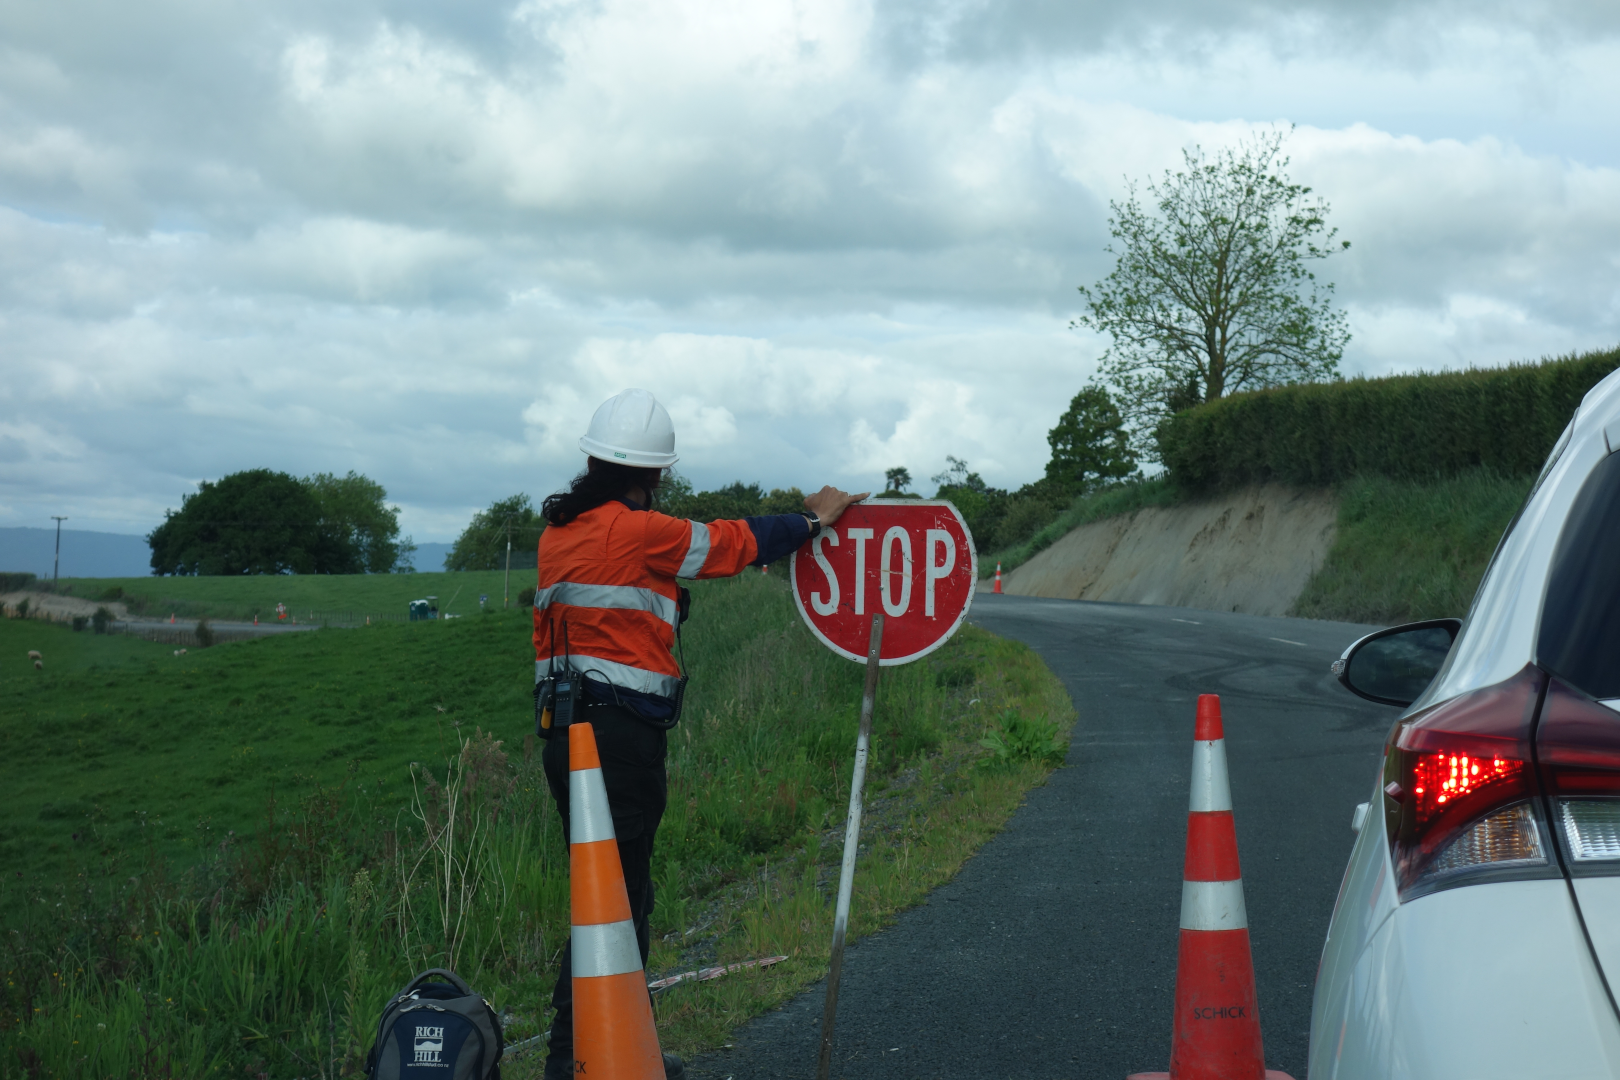
\includegraphics[height=\paperheight]{stop}
}
\begin{frame}[fragile]{\pc{\K{break}}, \pc{\K{continue}}}
  \pause
  \begin{java}
for (int i = 0; i < 0; ++i) {
    if (skipCondition)
        continue;
    // WORK
    if (stopCondition)
        break;
    // WORK
}
  \end{java}
  \pause
  \begin{center}
    \colbox[center, colalert]{À utiliser parcimonieusement !}
  \end{center}
\end{frame}
}

\subsection{Saisie utilisateur}
\begin{frame}
  \begin{block}{}
    Écrire un algorithme et un programme qui calcule et retourne
    la somme d’une série de nombres donnés par l’utilisateur.
  \end{block}

\end{frame}

\begin{frame}{Variante 1~: le nombre de valeurs est connu}
  \begin{block}{}
    Écrire un algorithme et un programme qui calcule et retourne
    la somme d’une série de nombres donnés par l’utilisateur.
  \end{block}

  L'utilisateur indique le nombre de termes au départ et rentre ensuite les
  termes.

  \pause
  On rendra l'entrée plus \og robuste \fg grâce à
  \begin{itemize}
    \item \pc{keyboard.hasNextInt();}\\
      qui lit un entier et retourne vrai ou faux selon que l'entrée est
      un entier.
    \item \pc{keyboard.next()} qui lit l'entrée, quelle qu'elle soit.
    \item \pc{keyboard.nextLine()} qui lit l'entièreté d'une ligne.
  \end{itemize}
\end{frame}

\begin{frame}{Variante 2~: demander à chaque fois s'il y a un suivant}
  \begin{block}{}
    Écrire un algorithme et un programme qui calcule et retourne
    la somme d’une série de nombres donnés par l’utilisateur.
  \end{block}

  À chaque itération, on demande à l'utilisateur s'il veut entrer un terme.
\end{frame}

\begin{frame}{Variante 3~: valeur sentinelle}
  \begin{block}{}
    Écrire un algorithme et un programme qui calcule et retourne
    la somme d’une série de nombres donnés par l’utilisateur.
  \end{block}

  On lit les nombres jusqu'à obtenir une valeur spéciale (par exemple -1)
  \pause ou (stop).

\end{frame}

\begin{frame}{Variante 4~: tout lire jusqu'à la fin du programme}
  \begin{block}{}
    Écrire un algorithme et un programme qui calcule et retourne
    la somme d’une série de nombres donnés par l’utilisateur.
  \end{block}

  On lit tous les nombres jusqu'à ce que l'entrée standard soit
  \structure{fermée} (avec \pc{Ctrl + D}).
\end{frame}


\section{Modules et références}
\frame{\sectionpage}

\subsection{Décomposer le problème}
\begin{frame}{Décomposer le problème}
  Jusqu'à maintenant, algorithmes d'un seul tenant.

  Dans la réalité, pour les problèmes plus conséquents, il faut décomposer
  en sous-problèmes. On adapte une \structure{structure modulaire}.

  \pause
  Cela permet de :
  \begin{itemize}
    \item libérer l'esprit;
    \item réutiliser ce qui a été fait;
    \item accroitre la lisibilité;
    \item répartir le travail en équipe.
  \end{itemize}

  \pause
  Un algorithme résolvant une partie d'un problème est appelé une
  \structure{fonction}, \structure{procédure}, \structure{méthode} ou
  \structure{module}.
\end{frame}

\begin{frame}[fragile]{Exemple}
\framesubtitle{Maximum de 3 nombres}
  \begin{center}
    \flowalgoddd{a (réel)}{b (réel)}{c (réel)}{max3}{réel}
  \end{center}

  \pause
  \vfill
  \begin{java}
public static double max3(double a, double b, double c) {
    if (a > b && a > c)
        return a;
    else if (b > c)
        return b;
    else
        return c;
}
  \end{java}
\end{frame}

\begin{frame}[fragile]{Exemple}
\framesubtitle{Maximum de 2 nombres}
  \begin{center}
    \flowalgodd{a (réel)}{b (réel)}{max2}{réel}
  \end{center}

  \pause
  \vfill
  \begin{java}
public static double max2(double a, double b) {
    if (a > b)
        return a;
    else
        return b;
}
  \end{java}
\end{frame}

\begin{frame}[fragile]{Exemple}
\framesubtitle{Maximum de 3 nombres --- modulaire}
  \begin{center}
  \begin{tikzpicture}[auto]
    \sffamily
    \node (a) at (0,4) {a (réel)};
    \node (b) at (0,2) {b (réel)};
    \node (c) at (0,0) {c (réel)};
    \node[draw,rounded corners] (max2a) at (2,3) {max2};
    \node[draw,rounded corners] (max2b) at (4,2) {max2};
    \node (r) at (6,2) {réel};
    \draw[rounded corners] (1,0) rectangle (5,4) node[above] {max3};
    \draw[->,thick] (a) to (max2a);
    \draw[->,thick] (b) to (max2a);
    \draw[->,thick] (c) to (max2b);
    \draw[->,thick] (max2a) to (max2b);
    \draw[->,thick] (max2b) to (r);
  \end{tikzpicture}
  \end{center}

  \pause
  \vfill
  \begin{java}
public static double max3(double a, double b, double c) {
    return max2(max2(a, b), c);
}
  \end{java}
\end{frame}

\subsection{Paramètres et valeur de retour}
\begin{frame}{Paramètres et valeur de retour}
  Jusqu'ici,
  \begin{itemize}
    \item paramètres d'un algorithme \(\sim\) données de l'algorithme;
    \item valeur unique de retour (\pc{\K{return}} de l'algorithme \(\sim\)
      résultat de l'algorithme.
  \end{itemize}

  \pause
  Mais il existe aussi :
  \begin{itemize}
    \item paramètres d'entrée;
    \item paramètres en entrée-sortie.
  \end{itemize}
\end{frame}

\begin{frame}{Valeur de retour}
  La \structure{valeur de retour} correspond au résultat de l'algorithme.

  \begin{minipage}{4.5cm}
    \begin{pseudocode}
      \LComment {Code appelant}
      \Decl{var}{integer}
      \Stmt var \Gets myAlgo()
      \Stmt myAlgo()
    \end{pseudocode}
  \end{minipage}
  \hfill
  \begin{minipage}{6.5cm}
    \begin{pseudocode}
      \LComment {Code appelé}
      \Algo{myAlgo}{}{integer}
      \Stmt \dots
      \EndAlgo
    \end{pseudocode}
  \end{minipage}

  \pause
  Un algorithme peut ne rien retourner.

  \pause
  S'il n'a pas de \Gives, il n'a pas de valeur et ne peut pas apparaitre dans
  une expression ou être assigné à une variable.

  \pause
  Nous contournerons le problème de valeur de retour unique plus tard
  (types composés, structures et objets).
\end{frame}

\begin{frame}[fragile]{Paramètre d'entrée}
  Le \structure{paramètre d'entrée} est une donnée de l'algorithme. Il ne peut
  pas être modifié\pause (pour l'appelant).

  Quand c'est nécessaire de le préciser, on le suit de \In.

  Ce paramètre est une \structure{valeur}.

  \vfill
  \begin{center}
  \begin{minipage}{4.5cm}
    \begin{pseudocode}
\LComment {Code appelant}
\Stmt myAlgo(expr)
\Empty
    \end{pseudocode}
  \end{minipage}
  \hfill
  \begin{minipage}{7cm}
    \begin{pseudocode}
\LComment {Code appelé}
\Algo{myAlgo}{\Par{par\In}{integer}}{}
\Stmt \dots
\EndAlgo
    \end{pseudocode}
  \end{minipage}
  \end{center}

  C’est comme si l’algorithme \pc{myAlgo} commençait par l’affectation
  \pc{par \Gets expr}.
\end{frame}

\begin{frame}[fragile]{Exemple}
  \begin{pseudocode}[1]
    \Algo{test}{}{} \RComment {Code appelant}
      \Decl {max}{real}
      \Let max \Gets max3(3, 2, 5)
      \Write max
    \EndAlgo
    \Algo{max3}{\Par{a\In, b\In, c\In}{reals}}{real}
      \RComment {Code appelé}
      \Decl{maxab, max}{reals}
      \Let maxab \Gets max2(a,b)
      \Let max \Gets max2(maxab,c)
      \Return max
    \EndAlgo
  \end{pseudocode}
\end{frame}

\begin{frame}{Exemple}
  \framesubtitle{trace}
  \begin{tabular}{|>{\centering\arraybackslash}m{1.1cm}
          |>{\centering\arraybackslash}m{13mm}
          |*{5}{>{\centering\arraybackslash}m{13mm}}|}
    \hline
    \rowcolor{black!50}
      & \pc{test} & \multicolumn{5}{c|}{\pc{max3}} \\
    \hline
    \rowcolor{black!30}
    \# & max  & {a} & {b} & {c} & {maxab} & {max}\\
    \hline
    2    & indéfini             &                      &                      &                      &                      &          \\
    3,6  & {\color{gray}$\mid$} & 3                    & 2                    & 5                    &                      &          \\
    7    & {\color{gray}$\mid$} & {\color{gray}$\mid$} & {\color{gray}$\mid$} & {\color{gray}$\mid$} & indéfini             & indéfini \\
    8    & {\color{gray}$\mid$} & {\color{gray}$\mid$} & {\color{gray}$\mid$} & {\color{gray}$\mid$} & 3                    & indéfini \\
    9   & {\color{gray}$\mid$} & {\color{gray}$\mid$} & {\color{gray}$\mid$} & {\color{gray}$\mid$} & {\color{gray}$\mid$} & 5        \\
    10,3 & 5                    &                      &                      &                      &                      &          \\
    \hline
  \end{tabular}
  \note{Deux fois var \pc{max}, mais c'est variables différentes !}
\end{frame}

\begin{frame}[fragile]{Paramètre en entrée-sortie}
  Le paramètre en \structure{entrée-sortie} est un paramètre tel que
  l'algorithme reçoit une valeur en entrée et il peut être modifié \pause
  (pour l'appelant).

  Quand c'est nécessaire de le préciser, on le suit de \InOut.

  \pause
  La modification de cette variable doit être visible par l'appelant. Ce
  paramètre, ou variable, doit être une \structure{référence} (passage
  par valeur vs par référence).

  \pause
  \begin{minipage}{4.5cm}
    \begin{pseudocode}
\LComment {Code appelant}
\Stmt myAlgo(variable)
\Empty
    \end{pseudocode}
  \end{minipage}
  \hfill
  \begin{minipage}{7cm}
    \begin{pseudocode}
\LComment {Code appelé}
\Algo{myAlgo}{\Par{par\In\Out}{entier}}{}
\Stmt \dots
\EndAlgo
    \end{pseudocode}
  \end{minipage}

  \pause
  Pas de \pc{\K{return}} nécessaire ici.
\end{frame}

\begin{frame}{Exemple}
  \begin{center}
    \flowalgov{nb (réel)}{valAbsolue}
  \end{center}

  \pause
  \begin{pseudocode}[1]
    \Algo{valAbsolue}{\Par{nb\In\Out}{réel}}{}
      \pause
      \If{nb < 0}
        \pause
        \Let nb \Gets -nb
        \pause
      \EndIf
    \EndAlgo
    \Algo{test}{}{}
    \Decl{température}{réel}
    \Let température \Gets -12.5
    \Stmt valAbsolue(température)
    \Write température
    \EndAlgo
  \end{pseudocode}
\end{frame}

\begin{frame}{Exemple}
  \framesubtitle{trace}
  \begin{center}
  \begin{tabular}{|>{\centering\arraybackslash}m{1cm}
          |>{\centering\arraybackslash}m{20mm}
          |*{2}{>{\centering\arraybackslash}m{20mm}}|}
    \hline
    \rowcolor{black!50}
      & \pc{test} & \multicolumn{2}{c|}{\pc{valAbsolue}} \\
    \hline
    \rowcolor{black!30}
    \# & température  & nb & test \\
    \hline
    8     & indéfini &  & \\
    9     & -12.5    &  & \\
    10, 1 & {\color{gray}$\mid$} & -12.5 & \\
    2     & {\color{gray}$\mid$} & {\color{gray}$\mid$} & vrai \\
    3     & {\color{gray}$\mid$} & 12.5 & \\
    5, 10 & 12.5 &  & \\
    \hline
  \end{tabular}
  \end{center}
\end{frame}

\subsection{Type primitif et type référence}
\begin{frame}{Type primitif et type référence}
  Paramètres en entrée et entrée-sortie, algorithmes vs programmation ? Dans
  les langages de programmation (supportant le concept de fonction) :
  \begin{itemize}
    \item tous acceptent d'avoir une valeur de retour unique;
    \item tous acceptent des paramètres en entrée;
    \item certains et sous certaines conditions acceptent des paramètres en
      entrée/sortie.
  \end{itemize}

  \pause
  Une histoire de \structure{type primitif} et \structure{type référence}.
\end{frame}

\begin{frame}{Type primitif}
  \begin{definition}
    Une variable de \structure{type primitif} est une variable qui contient
    directement la valeur qui lui est assignée.  Cette variable a une taille
    fixe qui dépend de son type. L'emplacement mémoire qui lui est attribué
    se trouve sur la \structure{pile} (\structure{\textit{stack}} en anglais).
  \end{definition}
  \note{
  Lorsqu'un programme s'exécute, le système lui attribue plusieurs
  emplacements mémoire~:un contenant les instructions et deux qui
  contiendront les variables du programme. La pile (\textit{stack}) et le
  tas (\textit{heap}).}

  \pause
  Par exemple, une variable de type \pc{int} a une taille de
  4~\textit{bytes} (32~bits).

  \begin{center}
  \begin{tikzpicture}
    \draw (0,0) rectangle (.7,.7);
    \draw (0,.7) node[above left]{\Large \texttt{i}};
    \draw (.35,.35) node{\Large 7};
  \end{tikzpicture}
  \end{center}

  Les types primitifs en Java sont \pc{\K{byte}}, \pc{\K{short}}
  \pc{\K{int}}, \pc{\K{long}}, \pc{\K{char}}, \dots
\end{frame}

\begin{frame}{Type référence}
  \begin{definition}[Type référence]
  Une variable de \structure{type référence} est une variable qui ne contient
  pas directement la valeur qui lui est assignée. Elle contient une adresse
  mémoire désignant l'endroit où est --- ou sera --- stockée la valeur.

  L'emplacement mémoire attribué à la variable se trouve sur la pile et
  a la même taille pour toutes les variables de type référence tandis
  que l'emplacement mémoire qui contiendra effectivement la valeur sera
  attribué sur le \structure{tas} (\structure{\textit{heap}} en anglais).
  \end{definition}

\end{frame}

\begin{frame}[fragile]
  \pc{String} est un type référence.

  \begin{java}
String s = "Hello";
s = "I would just like to say hello";
  \end{java}

  \only<1-2> {
  \hspace{3cm}
  \begin{tikzpicture}
    \node[draw, minimum width=.5cm,
      minimum height=.5cm,label={above:\texttt{s}}] (ref) {};
      \only<1>{\node[draw, below of=ref, right] (string) at (0,0) {Hello};}
      \only<1>{\draw[->] (ref.center) -- (string);}
      \only<2>{\node[draw, below of=ref, right] (string2) at (2,0) {I would
      just like to say hello};}
      \only<2>{\draw[->] (ref.center) -- (string2);}
  \end{tikzpicture}
  }

  \pause
  Il y a d'autres types référence en Java (vous connaissez déjà \pc{Scanner}).
\end{frame}

\begin{frame}{Paramètres en Java}
  En Java, les méthodes retournent avec \pc{\K{return} expression}. Une
  méthode peut ne rien retourner.

  En Java, les paramètres se passent \structure{par valeur}.
  \begin{itemize}
    \item Les types \structure{primitifs} en paramètre agissent comme des
      paramètres \structure{d'entrée}.
    \item Les types \structure{référence} en paramètre agissent comme des
      paramètres \structure{d'entrée-sortie} (sauf s'ils sont \pc{\K{final}}).
  \end{itemize}
\end{frame}

\begin{frame}
  \begin{definition}
    Les paramètres déclarés dans \structure{l'entête} d'un algorithme sont
    appelés les \structure{paramètres formels}.\\
    Les paramètres \structure{donnés à l'appel} de l'algorithme sont appelés
    \structure{paramètres effectifs}.
  \end{definition}
\end{frame}

\section[Documentation]{Documentation, Javadoc}
\frame{\sectionpage}

\begin{frame}{Plusieurs documentations}
\begin{description}
  \item[destinée à l'utilisateur] \(\sim\) manuel de l'utilisateur. Copies
    d'écrans, explications du fonctionnement du programme. Informations
    nécessaires à l'utilisation du programme.
  \item[destinée au développeur] explication des méthodes que le
    développeur peut être amené à utiliser.
    \pause
    \begin{itemize}[<+->]
      \item interne (fonctionnement du code)
      \item interface (API, \textit{Application Programming Interface})
    \end{itemize}
\end{description}
\end{frame}

\begin{frame}{Documentation développeur}
  Décomposer, factoriser, réutiliser du code\\
  \qquad \(\rightarrow\) beaucoup de méthodes à connaître.

  \pause
  Un développeur doit tout connaître ? \pause Non, il doit juste savoir
  chercher.

  \pause
  La documentation développeur doit être :
  \begin{itemize}[<+->]
    \item accessible/navigable rapidement;
    \item dans un format uniforme;
    \item maintenue.
  \end{itemize}

  \pause
  Malheureusement, souvent laissée de côté (par flemme ?).

  \pause
  Documentation API Java :\\
  \url{https://docs.oracle.com/en/java/javase/11/docs/api}

  \note{Montrer doc java.lang.Math, description de classe puis descriptions
  courtes puis descriptions longues.}

\end{frame}

\begin{frame}{Documentation dans le code}
  \framesubtitle{\textit{litterate programming}}
  \begin{itemize}[<+->]
    \item accompagne le code;
    \item écrite et mise à jour en même temps;
    \item suit une syntaxe particulière (c'est presque du code);
    \item extraite automatiquement par un outil pour en faire un document
      facile à lire;
    \item ce document --- quelle que soit la personne qui écrit la
      documentation --- suit la même structure, le même format, le même style
      et est donc facile à lire.
  \end{itemize}
\end{frame}

\subsection{Javadoc}
\begin{frame}[fragile]{\pc{Javadoc}}
  \begin{java}
    // Commentaire simple
    /* Commentaire
     * Multi-lignes */
    /**
     * Commentaire Javadoc
     */
  \end{java}

  \pause
  \structure{Commentaire Javadoc} placé \alert{au dessus} de la déclaration
  de classe/méthode qu'il documente.
\end{frame}

\begin{frame}[fragile]{\pc{Javadoc}}
  \begin{java}
/**
 * Description courte de la méthode terminée par un point.
 *
 * Un peu plus en détail ce que fait la méthode.
 * La description longue peut contenir des balises html
 * comme <strong>écrire en gras</strong> par exemple.
 *
 * @param par1 rôle du paramètre (son type est déduit)
 * @return valeur de retour
 */
public static <type> <nom>(<params>) {
    // Statement
}
  \end{java}
\end{frame}

\begin{frame}[fragile]{\pc{Javadoc}}
  \begin{itemize}
    \item Générée ``à la main''
      \begin{verbatim}
$ cd ~/NetBeansProjects/JavaApplication1/dev1-cours
$ javadoc -sourcepath src/main/java \
    -subpackages pha.dev1 -d doc/
      \end{verbatim}
    \item Via l'IDE (NetBeans) : Run \(\rightarrow\) Generate Javadoc\\
      (éventuellement, il faut Clean and Build Projet avant)
  \end{itemize}
\end{frame}

\begin{frame}{Tags}
  \structure{Tag} = mot commençant par un arobase @.\\
  Sert à spécifier une information formattée automatiquement.

  \pause
  Certains requis (par convention), certains optionnels.

  Documentation style Oracle:\\
  \url{https://www.oracle.com/technical-resources/articles/java/javadoc-tool.html}

  Documentation syntaxe :\\
  \url{https://docs.oracle.com/en/java/javase/11/docs/specs/doc-comment-spec.html}
\end{frame}
\begin{frame}{Tags}
  \begin{description}
    \item[@author] le ou les auteurs. Un \textit{tag}
      par auteur (peut-être un groupe/société). Ne génère pas
      de \textit{javadoc}, visible que dans la classe.
      (\textit{classes}, \textit{requis});
    \item[@version] date de modification et numéro de version
      commençant à 1.1.  (\textit{classes}, \textit{requis});

      \par Par exemple \textit{1.39, 1996-01-23}
    \item[@param] un par paramètre de méthode;
      (\textit{méthodes}, \textit{requis});
    \item[@return] ce que retourne la méthode;
      (\textit{méthodes}, \textit{requis} excepté si la méthode ne retourne rien);
    \item[@throws] listes les exceptions éventuellement lancées par la méthode;
      (\textit{méthodes});
    \item[@see] référence à une autre classe/méthode relative
      à ce qui est documenté.
  \end{description}
\end{frame}

\begin{frame}[fragile]{Style}
  \begin{enumerate}[<+->]
    \item Commenter seulement classes et méthodes \structure{publiques}.
    \item Dans la mesure du possible la \textit{javadoc} s'écrit en
      \structure{anglais}.
    \item Mots clés (\textit{keywords}), noms de classes, de méthodes :
      écrit dans un \structure{inline tag} \pc{\{@code foo bar\}}
    \item On préfèrera la $3^e$ personne à la $2^e$ personne.
    \seti
  \end{enumerate}
\end{frame}
\begin{frame}[fragile]{Style}
  \begin{enumerate}
    \conti
    \item Description de méthode commence par un verbe, parce qu'elle
      implémente habituellement une opération, une action.\\
      \medskip
      \quad\textit{Gets the label of this button.} \\
      sera préféré à \\
      \quad\textit{This method gets the label of this button.}
    \seti
  \end{enumerate}
\end{frame}
\begin{frame}[fragile]{Style}
  \begin{enumerate}
    \conti
    \item Ajouter le commentaire au nom de la méthode sans répéter le nom de la
      méthode. Inutile de répéter. \(\rightarrow\) Apporter une plus-value
      au nom de la méthode.\\
      \begin{wrong}
      \begin{java}
/**
  * Sets the tool tip text.
  *
  * @param text the text of the tool tip
  */
  public void setToolTipText(String text)
      \end{java}
      \end{wrong}
  \end{enumerate}
\end{frame}
\begin{frame}[fragile]{Style}
  \begin{enumerate}
    \conti
    \item Ajouter le commentaire au nom de la méthode sans répéter le nom de la
      méthode. Inutile de répéter. \(\rightarrow\) Apporter une plus-value
      au nom de la méthode.\\
      \begin{java}
/**
  * Registers the text to display in a tool tip.
  *
  * The text displays when the cursor lingers over
  * the component.
  *
  * @param text the string to display. If the text
  * is null, the tool tip is turned off for
  * this component.
  */
  public void setToolTipText(String text)
      \end{java}
    \seti
  \end{enumerate}
\end{frame}
\begin{frame}[fragile]{Style}
  \begin{enumerate}[<+->]
    \conti
    \item Le tag \texttt{@link} peut être utilisé… avec parcimonie car un lien
      attire l'attention. Il ne faut pas en abuser. Ce tag s'écrit dans le
      texte et fait référence vers l'API.

    \item Lorsqu'une référence à une autre méthode est faite, on omet les
      parenthèses \texttt{add} ou on écrit le type des paramètres
      \texttt{add(int, Object)} sans nom pour les paramètres.

    \item Lors de la description éventuelle d'une variable, omettre le sujet
      dans un souci de brièveté.\\
      \medskip
      \quad\textit{Counter of vowels}\\
      sera préféré à\\
      \quad\textit{This is a counter of vowels}.

    \item Éviter les abréviations non universelles.

  \end{enumerate}
\end{frame}

\section{Les types}
\begin{frame}{Tout est données (binaires)}
  En mémoire, tout n'est que séquence de 0 et 1.
  \begin{itemize}
    \item \pc{\K{True}} : \pc{1}
    \item \pc{\K{False}} : 0
    \item \pc{42} : 101010
    \item \pc{-1} : 11111111111111111111111111111111
    \item \pc{2.5} : {\small
      100000000000100000000000000000000000000000000000000000000000000}
    \item \(\pi\) : {\small
      100000000001001001000011111101101010100010001000010110100011000}
    \item \og Hello \fg : 10010001100101110110011011001101111
  \end{itemize}
\end{frame}

\begin{frame}{Tout a un type}
  Les opérations sur les données dépendent de leur \structure{type}.

  \pause
  \begin{itemize}
    \item Types primitifs (basiques)
    \item Types composés (complexes)
  \end{itemize}

  \pause
  \begin{definition}
    Une valeur écrite dans un programme est appelée un
    \structure{littéral}. Il a une \structure{valeur} et un \structure{type}.
  \end{definition}
\end{frame}

\subsection{Types primitifs}
\begin{frame}{Types primitifs}
  Ils sont manipulés \emph{directement} par l'ordinateur. Il y en a 8 en Java :
  \begin{itemize}
    \item \pc{boolean}
    \item \pc{byte} \pc{short} \pc{int} \pc{long} \pc{char}
    \item \pc{float} \pc{double}
  \end{itemize}

  \begin{center}
    \includegraphics[width=.7\linewidth]{\sybprffx/images/primitifs.pdf}
  \end{center}
\end{frame}


\begin{frame}{Types numériques entiers}
  Stockés en notation \structure{complément à deux}.

  Diffèrent par leur taille (en bits) en mémoire.

  \begin{tabular}[h]{|l|l|p{8cm}|}
    \hline
    \rowcolor{black!20}
    \textbf{Type}  &  \textbf{Taille}  &  \textbf{Intervalle}  \\
    \hline
    \pc{byte}  &  8 bits  &  [-128, 127]\\
        &      &  [$-2^7$, $2^7-1$]\\
    \pc{short}  &  16 bits  &  [-32\,768, 32\,767]\\
        &      &  [$-2^{15}$, $2^{15}-1$]\\
    \pc{int}    &  32 bits  &  [-2\,147\,483\,648, 2\,147\,483\,647]\\
        &      &  [$-2^{31}$, $2^{31}-1$]\\
    \pc{long}  &  64 bits
      &  \small{[-9\,223\,372\,036\,854\,775\,808,
      9\,223\,372\,036\,854\,775\,807]}\\
        &      &  [$-2^{63}$, $2^{63}-1$]\\
    \hline
  \end{tabular}
  \note{Parler de gangnam style qui a dépassé \(2^32\) vues et forcé Google a
    adapter le type de compteur de vues en long.}
\end{frame}

\begin{frame}[fragile]{Littéraux numérique entiers}
  \framesubtitle{décimal}
  \begin{itemize}[<+->]
    \item formé des chiffres \texttt{0123456789} et \texttt{\_};
    \item un littéral est de type \pc{int} ou \pc{long}, jamais de type
      \pc{byte} ou \pc{short};
    \item pour distinguer un littéral \pc{long}
      du type par défaut \pc{int}, suffixer d'un \texttt{l} ou \texttt{L};
  \end{itemize}

  \pause
  \begin{java}
int myInt = 42;
int myOtherIntSomeValue = 1_00;
long myLong = 42L;
  \end{java}
  \note{Ceci ne nous empêchera pas d'écrire \pc{byte b = 5} par exemple. Nous
    verrons les conversions en Développement II}

\end{frame}

\begin{frame}[fragile]{Littéraux numérique entiers}
  \framesubtitle{octal}
  \begin{itemize}
    \item les chiffres \texttt{01234567} et \texttt{\_};
    \item commence par un \texttt{0};
    \item un littéral est de type \pc{int} ou \pc{long}, jamais de type
      \pc{byte} ou \pc{short};
    \item pour distinguer un littéral \pc{long} du type par défaut \pc{int}, suffixer
      d'un \texttt{l} ou \texttt{L};
  \end{itemize}

  \pause
  \begin{java}
int myOctalInt = 052;
int anoherOctalInt = 01_44;
long myOctalLong = 0144L;
  \end{java}
  \note{Attention à \pc{010 + 1} = \dots \(9_{10}\)}
\end{frame}

\begin{frame}[fragile]{Littéraux numérique entiers}
  \framesubtitle{hexadécimal}
  \begin{itemize}
    \item les chiffres \texttt{0123456789ABCDEFabcdef} et \texttt{\_};
    \item commence par un \texttt{0x} ou \texttt{0X};
    \item un littéral est de type \pc{int} ou \pc{long}, jamais de type
      \pc{byte} ou \pc{short};
    \item pour distinguer un littéral \pc{long} du type par défaut \pc{int}, suffixer
      d'un \texttt{l} ou \texttt{L};
  \end{itemize}

  \pause
  \begin{java}
int myHexadecimalInt = 0x64;
int anotherHexadecimalInt = 0x2A;
long myHexadecimalLong = 0X64l;
  \end{java}
\end{frame}

\begin{frame}[fragile]{Littéraux numérique entiers}
  \framesubtitle{binaire}
  \begin{itemize}
    \item les chiffres \texttt{01} et \texttt{\_};
    \item commence par un \texttt{0b} ou \texttt{0B};
    \item un littéral est de type \pc{int} ou \pc{long}, jamais de type
      \pc{byte} ou \pc{short};
    \item pour distinguer un littéral \pc{long} du type par défaut \pc{int}, suffixer
      d'un \texttt{l} ou \texttt{L};
  \end{itemize}

  \pause
  \begin{java}
int myBinaryInt = 0b101010;
int anotherBinaryInt = 0b01100100;
int yetAnotherBinaryInt = 0B0110_0100;
  \end{java}
  \note{Dire que toujours même valeur dans les variables.

  Print ne dépend pas de la représentation utilisée pour le litéral.}
\end{frame}

\begin{frame}{Littéraux numériques entier \pc{\K{char}}}
  Représente un \structure{caractère} (\textit{character}).
  Litéral '\pc{a}'.

  Entier non signé de 16~bits représentant le code Unicode codé en UTF-16
  du caractère.

  \begin{center}
  \begin{tabular}[h]{|l|l|p{9cm}|}
    \hline
    \rowcolor{black!20}
    \textbf{Type}  &  \textbf{Taille}  &  \textbf{Intervalle}  \\
    \hline
    \pc{char}  &  16 bits  &  [0, 65\,535]\\
    &      &  [$0$, $2^{16}-1$]\\
    \hline
  \end{tabular}
  \end{center}

  \pause
  Les caractères peuvent être \structure{échappés} (\structure{échappement de
  caractères}) :
  \begin{multicols}{2}
    \begin{itemize}
      \item '\pc{\textbackslash n}' : retour à la ligne
      \item '\pc{\textbackslash r}' : retour chariot
      \item '\pc{\textbackslash t}' : tabulation
      \item '\pc{\textbackslash}'\,' : déspécialisation du '
      \item '\pc{\textbackslash "}' : déspécialisation du "
    \end{itemize}
  \end{multicols}
\end{frame}

\begin{frame}{Les types primitifs numériques à virgule flottante}
  Nombres \structure{pseudo-réels} ou à \structure{virgule flottante}.
  \[nombre = (\pm 1) \cdot mantisse \cdot 2^{exposant}\]
  \begin{center}
  \begin{tabular}[t]{|l|c|c|c|c|}
    \hline
    \rowcolor{black!40}
    \textbf{Type}   & \textbf{Taille (\textit{bit})}
    & \textbf{Exposant} & \textbf{Mantisse} & \textbf{Intervalle}\\
    \hline
    float  & 32 bits          & 8    & 23 &
    [\(1.4 \cdot 10^{-45}, 3.4 \cdot 10^{38}\)]\\
    \hline
    double  & 64 bits          & 11  & 52 &
    [\(4.9 \cdot 10^{-324}, 1.8 \cdot 10^{308}\)]\\
    \hline
  \end{tabular}
  \end{center}
\end{frame}

\begin{frame}{Littéraux numériques à virgule flottante}
  Écrit en base 10.
  \begin{center}
    \bf \pc{| entier | . | décimales | exposant | suffixe
    |}
  \end{center}
  \begin{itemize}
    \item \pc{entier} : chiffres avant la virgule (\pc{\_} autorisé);
    \item \pc{.} : séparateur décimales;
    \item \pc{décimales} : chiffres après la virgule;
    \item \pc{exposant} : \pc{e} ou \pc{E} suivi d'un entier,
      l'exposant (puissance de 10);
    \item \pc{suffixe} : \pc{f}, \pc{F}, \pc{d} ou \pc{D}, spécifie si c'est un
      \pc{float} ou un \pc{double} (par défaut \pc{double}).
  \end{itemize}
\end{frame}

\begin{frame}[fragile]{Littéraux numériques à virgule flottante}
  \framesubtitle{en base 10}
\begin{java}
double myDouble;
myDouble = 1.;       // 1.0
myDouble = .1;       // 0.1
myDouble = 1e1;      // 10.0
myDouble = 1d;       // 1.0
myDouble = 1.e0;     // 1.0
myDouble = 1_000.45; // 1000.45
myDouble = 1.45e3;   // 1450.0
myDouble = .45e3d;   // 450.0

float myFloat;
myFloat = 1f;      // 1.0
myFloat = 1.f      // 1.0
\end{java}
\end{frame}

\begin{frame}{Littéraux numériques à virgule flottante}
  Écrit en base 16.
  \begin{center}
    \bf \pc{| entier | . | décimales | exposant | suffixe
    |}
  \end{center}
  \begin{itemize}
    \item débute par \pc{0x} ou \pc{0X};
    \item \pc{entier} : chiffres avant la virgule (\pc{\_} autorisé);
    \item \pc{.} : séparateur décimales;
    \item \pc{décimales} : chiffres après la virgule;
    \item \pc{exposant} : \pc{p} ou \pc{P} suivi d'un entier,
      l'exposant (puissance de 2);
    \item \pc{suffixe} : \pc{f}, \pc{F}, \pc{d} ou \pc{D}, spécifie si c'est un
      \pc{float} ou un \pc{double} (par défaut \pc{double}).
  \end{itemize}
\end{frame}

\begin{frame}[fragile]{Littéraux numériques à virgule flottante}
  \framesubtitle{en base 16}
\begin{java}
  double myDouble;
  myDouble = 0x1p0;    // 1.0 = 1 * 2^0
  myDouble = 0x1.1p0;  // 1.0625 = 1 + (1/16)
  myDouble = 0x1p1;    // 2.0 = 1 * 2^1
  myDouble = 0xA.Bp0;  // 10.6875= 10 + 11*1/16
  myDouble = 0x1E2p2;  // 1928 = (1*16^2 + 14*16^1 + 2*16^0) * 2^2

  float myFloat;
  myFloat = 0X.1p4f;   // 1.0 = (1*16^-1) * 2^4
\end{java}
\end{frame}

\begin{frame}[fragile]{Primitif booléen}
  Un \structure{booléen} est \structure{vrai} ou \structure{faux}.

  Ses littéraux \pc{true} et \pc{false}.

\begin{java}
boolean myBoolean = true;
boolean anotherBoolean = false;
\end{java}
\end{frame}

\subsection{Types référence}
\begin{frame}{Types référence}
  En java, \structure{type composés/complexes} = \structure{types référence}.

  Exemples : \pc{String}, \pc{Scanner}, \pc{Random}, les \textit{tableaux}.
  \note{Reparler de référence, allocation stack, heap, avec dessin boite};
\end{frame}

\begin{frame}[fragile]{Littéraux de type \pc{String}}
  Chaîne de caractères (\pc{String}) : texte entouré de guillemets doubles
  (\textit{double quote}).
  \begin{java}
String myString = "Hello";
String anotherString = "Hello \n World";
  \end{java}
\end{frame}

\begin{frame}[fragile]{Littéraux de type \pc{String}}
  Deux littéraux identiques sont alloués \alert{une seule} fois.
  \begin{java}
String s1 = "Hello";
String s2 = "Hello";
  \end{java}

  \begin{center}
    \begin{tikzpicture}
      \node[draw, minimum width=.5cm,
        minimum height=.5cm,label={above:\texttt{s1}}] (ref1) {};
      \node[draw, minimum width=.5cm,
        minimum height=.5cm,label={above:\texttt{s2}}] (ref2) at (1,0) {};
      \node[draw, below of=ref2, right] (string) at (2,-0.5) {Hello};
      \draw[->] (ref1.center) -- (string);
      \draw[->] (ref2.center) -- (string);
    \end{tikzpicture}
  \end{center}
  \note{Exemple compute str -> pas égales, avec equals.}
\end{frame}

\begin{frame}{Durée de vie}
  \begin{definition}
    La \structure{durée de vie} (\textit{\structure{lifetime}}) d'une variable
    est la période de temps pendant laquelle les données de la variable
    sont dans un état valide / accessible.
  \end{definition}

  Pour les variables locales (non statiques), le \structure{lifetime} est
  généralement limité au \structure{scope} (portée).

  Dans d'autres cas (p.ex : lecture d'un \pc{String} au clavier), cela
  dépend du langage :
  \begin{itemize}
    \item il faut explicitement gérer (et libérer) la mémoire allouée;
    \item le langage (Java) se charge de la gestion mémoire. Un
      \structure{ramasse-miette} (\textit{\structure{garbage collector}})
      parcourt \og régulièrement \fg la mémoire afin de libérer les espaces
      mémoire non référencés.
  \end{itemize}
\end{frame}

\section{String}
\frame{\sectionpage}

\begin{frame}{\pc{String}}
  Chaine de caractères (\pc{String}) = séquence de caractères (\pc{char}).

  \vfill
  \begin{center}
  \begin{tabular}[c]{*{5}{|c}|}
    \hline
    \pc{H} & \pc{e} & \pc{l} & \pc{l} & \pc{o}\\
    \hline
    \multicolumn{1}{c}{0} & \multicolumn{1}{c}{1} & \multicolumn{1}{c}{2} &
    \multicolumn{1}{c}{3} & \multicolumn{1}{c}{4}
  \end{tabular}
  \end{center}

  \vfill
  \begin{center}
    '\pc{A}' \(\neq\) \pc{"A"}
  \end{center}
\end{frame}

\begin{frame}[fragile]{Longueur}
  \begin{java}
"Bonjour".length();  // -> 7.
"Une chaine".length();  // -> 10 (l'espace compte pour 1).
"A".length();  // -> 1.
"".length(); // -> 0.
String someString = "Hello there !";
someString.length(); // -> 13
  \end{java}
\end{frame}

\begin{frame}[fragile]{Contenu d'une chaine}
  \begin{center}
  \begin{tabular}[c]{*{7}{|c}|}
    \hline
    \pc{B} & \pc{o} & \pc{n} & \pc{j} & \pc{o} & \pc{u} & \pc{r}\\
    \hline
    \multicolumn{1}{c}{0} & \multicolumn{1}{c}{1} & \multicolumn{1}{c}{2} &
    \multicolumn{1}{c}{3} & \multicolumn{1}{c}{4} & \multicolumn{1}{c}{5} &
    \multicolumn{1}{c}{6}
  \end{tabular}
  \end{center}

  \vfill
  \begin{java}
char c = "Bonjour".charAt(2);  // le caractère 'n'
  \end{java}

  \vfill
  \pause
  \begin{block}{Exercice}
    Écrire un algorithme qui vérifie si un mot contient une lettre donnée.
  \end{block}
\end{frame}

\begin{frame}{Exercice}
  \begin{block}{Exercice}
    Écrire un algorithme qui retourne la position d'une lettre donnée dans
    un mot.
  \end{block}
  \begin{block}{Exercice}
    Écrire un algorithme qui vérifie si un mot en contient un autre.
  \end{block}
  \begin{block}{Exercice}
    Écrire un algorithme qui retourne la position d'un sous-mot dans
    un mot donné.
  \end{block}
\end{frame}

\begin{frame}[fragile]{Digression --- Surcharge de méthode}
  La \structure{surcharge de méthode} (\textit{\structure{method
  overloading}}) apparait quand on définit plusieurs méthodes avec le
  même nom mais des paramètres différents (en types ou en nombre).

  \begin{java}
    int max(int a, int b) { ... }
    int max(int a, int b, int c) { ... }
    double max(double a, double b) { ... }
    double max(double a, double b, double c) { ... }
  \end{java}
  \note{Implémenter tout ça}
\end{frame}

\begin{frame}[fragile]{Concaténation}
  Rassembler plusieurs chaines en une = \structure{concaténation}.

  En java, l'opérateur de concaténation est \pc{+} quand les opérandes
  sont des \pc{String}.

  \begin{java}
String text;
text = "al" + "go" + "rithmique";
  \end{java}
\end{frame}

\begin{frame}[fragile]{Concaténation}
  \begin{block}{Exercice}
    Écrire un algorithme qui inverse toutes les lettres d'un mot.
    Ainsi, "algo" deviendra "ogla".
  \end{block}

  \pause
  \begin{java}
public static String mirror(String word) {
    String mirror = "";
    for (int i = 0; i < word.length(); ++i) {
        mirror = word.charAt(i) + mirror;
    }
    return mirror;
}
  \end{java}
\end{frame}

\begin{frame}[fragile]{Concaténation}
  Concaténations succéssives inefficace.

  \pause
  Ici, il vaut mieux utiliser un \pc{StringBuilder}
  \begin{java}
public static String mirror(String word) {
    StringBuilder sb = new StringBuilder(word);
    for (int i = 0; i < word.length(); ++i) {
        int c = word.charAt(i);
        sb.setCharAt(word.length() - i - 1, c);
    }
    return sb.toString();
}
  \end{java}
\end{frame}

\begin{frame}{Manipuler les caractères --- API}
  L'API définit un tas de méthodes dans \pc{Character} et \pc{String} pour
  manipuler les caractères.
  \begin{description}
    \item \structure{\pc{isLetter}}
    \item \structure{\pc{isLowerCase}}
    \item \structure{\pc{isUpperCase}}
    \item \structure{\pc{isDigit}}
    \item \structure{\pc{toUpperCase}}
    \item \structure{\pc{toLowerCase}}
  \end{description}
\end{frame}

\begin{frame}[fragile]{Alphabet}
  \framesubtitle{lettre vers indice}
  \begin{block}{Problème}
    Écrire une méthode \pc{letterIndex} qui retourne un entier entre 1 et 26
    représentant l'indice d'une lettre (indépendament de sa casse).\\
    Par exemple, \pc{letterIndex('e')} \(\rightarrow\) 5,\\
    mais aussi \pc{letterIndex('E')} \(\rightarrow\) 5.
  \end{block}

  \pause Le code de la lettre '\pc{A}' dans le charset UTF-16 est 65 (0x0041),
  et celui de '\pc{a}' est 97 (0x0061).

  \pause
  \begin{java}
public static int letterIndex(char c) {
    return Character.toLowerCase(c) - 'a' + 1;
}
  \end{java}
\end{frame}

\begin{frame}[fragile]{Alphabet}
  \framesubtitle{lettre vers indice}
  Et si on veut gérer les caractères accentués ?
  \pause
  \begin{java}
public static int letterIndex(char c){
    c = Normalizer
            .normalize(""+c, Normalizer.Form.NFD)
            .replaceAll("[\u0300-\u036F]", "")
            .charAt(0);
    return Character.toLowerCase(c) - 'a' + 1;
}
  \end{java}
\end{frame}

\begin{frame}[fragile]{Alphabet}
  \framesubtitle{indice vers lettre}
  \begin{block}{Problème}
    Écrire une méthode \pc{indexToUpperChar} qui retourne le charactère
    (majuscule) correspondant au numéro d'une lettre.\\
    Par exemple, \pc{indexToUpperChar(5)} \(\rightarrow\) 'e',
  \end{block}
  \pause
  \begin{java}
public static char indexToUpperChar(int i) {
    return 'A' + n - 1;
}
  \end{java}
  \begin{java}
public static char indexToLowerChar(int i) {
    return 'a' + n - 1;
}
  \end{java}
\end{frame}

\begin{frame}[fragile]{Chaine et nombre}
  \framesubtitle{Nombre vers chaine}
  Conversions de nombres en chaine implicites :
  \begin{java}
String s = 42;
  \end{java}

  \pause Attention à l'ordre d'évaluation des opérandes.
  \begin{itemize}
    \item \pc{String s1 = 1 + "2"} \pause \(\rightarrow\) "12"
    \pause
    \item \pc{String s2 = 1 + 2} \pause \(\rightarrow\) "3"
    \pause
    \item \pc{String s3 = 1 + "2" + "3"} \pause\(\rightarrow\) "123"
    \pause
    \item \pc{String s4 = 1 + 2 + "3"} \pause \(\rightarrow\) "33"
  \end{itemize}
\end{frame}

\begin{frame}[fragile]{Chaine et nombre}
  \framesubtitle{Chaine vers nombre}
  Pour chaque type numérique, une méthode qui transforme le nombre en chaine de
  caractères.
  \begin{java}
String s = "3.14";
double d = Double.parseDouble(s);
s = "5";
int i = Integer.parseInt(s);
  \end{java}
\end{frame}

\begin{frame}[fragile]{Extraction de sous-chaine}
  Extraction d'une sous-chaine à partir d'un indice de caractère, jusqu'à un
  autre, exclu.
  \begin{java}
String s = "Hello there !";
System.out.println(s.substring(6,11));
String s2 = "15/10/2020";
int d = Integer.parseInt(s2.substring(0, 2));
int m = Integer.parseInt(s2.substring(3, 5));
int y = Integer.parseInt(s2.substring(6, 10));
System.out.println(d + "-" + m + "-" + y);
  \end{java}
\end{frame}

\section{Exceptions}
\frame{\sectionpage}

\begin{frame}[fragile]{Exceptions}
  Un programme ne doit jamais planter.

  \pause
  Toutes les erreurs ne sont pas des erreurs de programmation. Elles peuvent
  être liées à une situation \structure{exceptionnelle} dans l'environnement
  du programme.

\begin{java}
import java.util.Scanner;
public class Affiche {
    public static void main(String[] args) {
        Scanner clavier = new Scanner(System.in);
        int nb = clavier.nextInt();
        System.out.println(nb);
    }
}
\end{java}
\end{frame}

\begin{frame}{Exemples d'exceptions}
\begin{description}
  \item[InputMismatchException] par exemple lorsque l'utilisateur ou
    l'utilisatrice entre une valeur qui n'est pas du type attendu\,;
  \item[ArrayIndexOutOfBoundException] par exemple lorsque le programme
    essaie d'accéder à un élément d'un tableau hors de celui-ci\,;
  \item[IllegalArgumentException] par exemple lorsque l'argument passé à
    une méthode n'est pas dans la plage des valeurs attendues\,;
  \item[NullPointerException] par exemple lorsque l'on essaie d'accéder à
    un tableau qui n'a pas été créé.
\end{description}
\end{frame}

\subsection{\pc{try-catch}}
\begin{frame}[fragile]{Attraper une exception}
  Une exception non gérée arrête l'exécution du programme.
  \pause Il faut gérer les exceptions. On parle de les \structure{intercepter}
  ou des les \structure{attraper} (\textit{\structure{catch}}). Pour cela, on
  utilise une instruction \pc{\K{try-catch}}.

  \begin{itemize}
    \item \pc{\K{try}} : contient les instructions qui \emph{peuvent mal se
      passer}\,;
    \item \pc{\K{catch}} : contient le code qui est \emph{en charge} de gérer
      le problème.
  \end{itemize}

  \begin{grammaire}
\grammarrule{TryStatement :}
    try \grammarrule{Block} \grammarrule{CatcheClauses}

\grammarrule{CatchClause :}
    catch ( \grammarrule{Type Identifier} ) \grammarrule{Block}
  \end{grammaire}
\end{frame}

\begin{frame}[fragile]{Attraper une exception}
  Quand une exception est levée dans un \pc{try}~:
  \begin{itemize}
    \item le code du \pc{\K{try}} est interrompu\,;
    \item le code du \pc{\K{catch}} est exécuté\,;
    \item l'exécution reprend après le bloc \pc{\K{try-catch}}.
  \end{itemize}
  \begin{java}
Scanner clavier = new Scanner(System.in);
try {
    int nb = clavier.nextInt();
    System.out.println(nb);
}
catch(InputMismatchException e) {
    System.out.println("Ce n'est pas un entier!");
}
  \end{java}
\end{frame}

\subsection{\pc{throw}}
\begin{frame}[fragile]{Lancer une exception}
  \framesubtitle{Fail early, fail loudly}

  Vos algorithmes peuvent \structure{lancer} des exceptions.

  \pause
  On utilise l'instruction \structure{\pc{\K{throw}}}.

  \pause
  \begin{grammaire}
\grammarrule{ThrowStatement :}
    throw \grammarrule{Expression};
  \end{grammaire}
\end{frame}

\begin{frame}[fragile]{Exemple}
  \framesubtitle{vérifier les arguments reçus}

\begin{java}
/**
 * Calcule la racine carrée d'un nombre.
 * @param nb le nombre dont on veut la racine carée.
 * @return la racine carrée de <code>nb<\code>.
 * @throws IllegalArgumentException si <code>nb</code> est négatif.
 */
public static double racineCarrée(double nb) {
    if (nb < 0) {
        throw new IllegalArgumentException(
            "nb doit être positif!");
    }
    // Traitement normal.
    // On est sûr que le paramètre est OK.
}
\end{java}
\end{frame}

\begin{frame}[fragile]{Exemple}
  \framesubtitle{vérifier les arguments reçus}
\begin{java}
try {
    System.out.println(racineCarrée(val));
} catch (IllegalArgumentException ex) {
    System.out.println("Calcul impossible !");
}
\end{java}
\end{frame}

\section{Tests}
\frame{\sectionpage}

\begin{frame}{Différents types d'erreurs}
  Un programme qui \textbf{tourne} n'est \textbf{pas} un programme
  \textbf{correct}.

  \pause
  Plusieurs types d'erreur :
  \begin{itemize}[<+->]
    \item erreurs de compilation;
    \item erreurs d'exécution
      \begin{itemize}
        \item qui arrête le programme;
        \item comportement anormal du programme;
      \end{itemize}
    \item erreur de programmation résultant en une inefficience (CPU/mémoire).
  \end{itemize}
\end{frame}

\begin{frame}{Garantir un niveau de qualité}
  Il faut que le programme fournisse un bon résultat dans tous les cas :
  \begin{itemize}[<+->]
    \item les cas généraux;
    \item les cas particuliers;
    \item lors d'une défaillance de l'environnement;

      Par exemple, si un capteur de distance est défectueux, il faut que la
      chaine de production s'arrête.

    \item lors d'une utilisation non conforme du programme.
  \end{itemize}

  \pause
  En plus d'une bonne analyse et d'un bon design, on implémente des
  \structure{tests unitaires}, d'intégration, fonctionnels, de
  non-régression, etc.
\end{frame}

\begin{frame}{Tests unitaires}
  \begin{definition}[Test unitaire]
    Procédure permettant de tester le bon fonctionnement d'une unité de
    code, une méthode \bsc{Java} dans notre cas.
  \end{definition}

  En fonction des paramètres qu'elle reçoit en entrée, la méthode
  fournit elle les bons résultats~?

  \pause
  Pour tester régulièrement --- très régulièrement --- notre programme nous avons
  besoin d'outils qui vont automatiser ces tests.
\end{frame}

\subsection{Planifier les tests}
\begin{frame}{Planifier les tests}
  Rappel :
  \begin{enumerate}
    \item spécifier le problème;
    \item fournir des exemples;
    \item écrire un algorithme;
    \item vérifier les exemples (en traçant l'algorithme);
    \item écrire un programme exécutable correspondant à l'algorithme;
    \item tester le programme et constater qu'il fournit bien les résultats attendus.
  \end{enumerate}

  Exemples = \structure{plan de tests}.
\end{frame}

\begin{frame}
  \begin{definition}[Plan de test]
    Liste ou un tableau d'exemples mettant en œuvre la méthode testée sur
    des cas variés et permettant de faire apparaitre des problèmes lors
    de l'exécution automatique.

    Chacun des tests sera défini par une méthode qui porte un nom
    qui explique l'objectif du test.
  \end{definition}

  \pause
  Les cas sont des cas généraux, mais aussi des cas testant des erreurs
  de programmation fréquentes :
  \begin{itemize}
    \item commencer ou arrêter trop tôt ou trop tard une boucle;
    \item ne pas initialiser ou mal initialiser une variable;
    \item confondre < et $\le$ ou > et $\ge$\dots voire < et >;
    \item confondre ET et OU;
    \item mal écrire la négation d'une proposition;
  \end{itemize}

  \note{
    Autant que possible, ce nom décrit
    aussi la portée ou le contexte de ce qui est vérifié.

    Parler de test driven development.

    Question d'expérience.
  }
\end{frame}

\subsection{Framework de test}
\begin{frame}{Tester automatiquement}
  Un changement dans une méthode pourrait amener une erreur dans une autre.

  \pause
  Tester \structure{tout} et \structure{souvent} (tout le temps).

  \pause
  Vous risquez d'oublier, d'avoir la flemme \(\rightarrow\) automatiser.

  \pause
  Utilisation d'un \structure{Framework de test}.

\end{frame}

\begin{frame}[fragile]{JUnit}
  Nous utiliserons \structure{JUnit}, un \textit{\structure{framework}} pour
  l'écriture de tests répétables.

  \pause
  N'est pas fourni avec le JDK, il faut l'installer
  (\href{http://junit.org}{junit.org}). Mais est fourni avec NetBeans.

  \pause
  Pour tester \texttt{MyClass.foo},
  il faut écrire une classe \texttt{MyClassTest}.
  Le nom de la classe de test porte le nom de la classe qu'elle teste,
  suffixé par \texttt{Test}.

  Ensuite, demander à JUnit d'exécuter
  cette classe. Clic dans IDE ou commande :
  \begin{term}
java org.junit.runner.JUnitCore \textbackslash
    my.package.MyClassTest
\end{term}
\end{frame}

\begin{frame}[fragile]{JUnit}

  La classe \texttt{MyClassTest} contient plusieurs méthodes. Une méthode de test
  par cas. Une méthode de test~:
  \begin{itemize}
    \item est autonome. Elle ne reçoit pas de paramètre et ne retourne rien;
    \item est précédée de l'annotation \pc{@Test} permettant de la faire
          reconnaitre comme un test unitaire;

    \item n'a pas de mot clé \pc{static}.
    \end{itemize}
\end{frame}

\begin{frame}[fragile]{JUnit}
  \begin{itemize}
    \item contient des affirmations qui seront évaluées;

      \textit{La méthode doit me retourner «~vrai~».}~: \pc{assertTrue()}\\
      \textit{La méthode doit me retourner «~faux~».}~: \pc{assertFalse()}\\
      \textit{La méthode doit me donner cette valeur si ses paramètres sont
      ceux-ci.}~:\\
      \pc{assertEquals(<valeur attendue>, <valeur>)}

                Ces trois méthodes \pc{assertTrue}, \pc{assertFalse}, \pc{assertEquals} sont définies dans la classe \pc{org.junit.Assert}.
                On peut les utiliser directement après les avoir préalablement importées :
\begin{java}
import static org.junit.Assert.*;
\end{java}
  \end{itemize}
\end{frame}

\end{hideedit}
\section{Tableaux}
\frame{\sectionpage}

\begin{frame}{Exemple préliminaire}
  \framesubtitle{Statistiques de ventes}
    \begin{quote}
      Un gérant d’une entreprise commerciale souhaite connaitre l’impact
      d’une journée de promotion publicitaire sur la vente de dix de ses
      produits.

      Pour ce faire, les numéros de ces produits (numérotés de
      0 à 9 pour simplifier) ainsi que les quantités vendues pendant cette
      journée de promotion sont encodés au fur et à mesure de leurs
      ventes.  En fin de journée, le vendeur entrera la valeur -1 pour
      signaler la fin de l’introduction des données.  Ensuite, les
      statistiques des ventes seront affichées.
    \end{quote}
    Voir implémentation \pc{exemples/SalesStatsSwitch.java}
\end{frame}

\begin{frame}{Statistiques de ventes}
  Et s'il y a 1000 produits différents ?

  \pause
  On utilise des \structure{tableaux} (\textit{\structure{arrays}}) comme des sortes \structure{variables
  indicées}.

  \pause
  Pas 10 compteurs, mais \textbf{une} variable \pc{cpt} compartimentée en 10
  \structure{éléments}.

  \begin{center}
    \setlength{\tabcolsep}{0pt}
    \begin{tabular}{*{7}{>{\centering\arraybackslash}m{4em}}}
      {} &
      \pc{cpt[0]} &
      \pc{cpt[1]} &
      \pc{cpt[2]} &
      \dots &
      \pc{cpt[8]} &
      \pc{cpt[9]}\\
      \hhline{~*{6}{-}}
      \multicolumn{1}{c|}{\pc{cpt}~} &
      \multicolumn{1}{c|}{~} &
      \multicolumn{1}{c|}{~} &
      \multicolumn{1}{c|}{~} &
      \multicolumn{1}{c|}{\dots} &
      \multicolumn{1}{c|}{~} &
      \multicolumn{1}{c|}{~}\\
      \hhline{~*{6}{-}}
    \end{tabular}
  \end{center}

  \pause Voir implémentation \pc{exemples/SalesStatsArray.java}
\end{frame}

\begin{frame}{Tableaux}
  \begin{block}{Définitions}
    \begin{description}[<+->]
      \item[Tableau]
        Suite d’éléments de même type portant tous le même nom mais se
        distinguant les uns des autres par un indice.
      \item[Indice]
        Entier
        donnant la position d’un élément dans la suite.\\
        Cet indice varie entre la position du premier élément
        et la position du dernier élément (bornes de l’indice).\\
        Notons qu’il n’y a pas de \og trou \fg:
        tous les éléments existent entre le premier et le dernier indice.
      \item[Taille]
        Nombre d'éléments d'un tableau.\\
        Attention, la taille est déterminée à la création du
        tableau et ne peut être modifiée pendant l'exécution.
    \end{description}
  \end{block}

  Un tableau est de type \structure{référence}.
\end{frame}

\begin{frame}{Création de tableau}
  Afin de pouvoir utiliser un tableau, il sera nécessaire de distinguer :
  \begin{itemize}
    \item la \structure{déclaration} qui consiste à signaler qu'une
      variable est un tableau. Dans un programme, cette déclaration
      a pour effet de réserver un emplacement mémoire qui contiendra
      une référence vers les cases du tableau\,;

    \item la \structure{création} du tableau consiste a réserver
      l'emplacement mémoire qui contiendra les différentes valeurs.
      Pour le créer, il faut connaitre sa taille\,;

    \item l'\structure{initialisation} du tableau consiste à donner ses
      premières valeurs aux différents éléments du tableau.

  \end{itemize}
\end{frame}

\begin{frame}[fragile]{Déclaration}
  Pour \structure{déclarer} un tableau :

\begin{grammaire}
\grammarrule{ArrayDeclarationStatement:}
    \grammarrule{Type}[] \grammarrule{Identifier}
\end{grammaire}

\begin{java}
int[] myArray;
String[] strings;
\end{java}

  \pause
  C'est juste une déclaration. Pas de mémoire allouée pour \textbf{contenir} les
  éléments du tableau.

\end{frame}

\begin{frame}[fragile]{Création}
  Pour \structure{créer} un tableau, préalablement déclaré, nous écrirons :
\begin{grammaire}
\grammarrule{ArrayCreationExpression:}
    new \grammarrule{Type}[\grammarrule{Expression}]
\end{grammaire}

\begin{java}
myArray = new int[10];
strings = new String[3];
\end{java}

  \pause
  L'emplacement mémoire nécessaire pour stocker la valeur de chaque élément
  du tableau est \structure{réservé} (\structure{alloué}).
\end{frame}

\begin{frame}[fragile]{Initialisation}
  Pour \structure{initialiser} les éléments du tableau, nous pouvons le faire en
  accédant à chaque élément du tableau. Un par un.

  L'accès aux éléments d'un tableau se fait grâce aux crochets
  \pc{myArray[i]} :
\begin{java}
myArray[0] = 5;
strings[1] = "Hello";
\end{java}
\end{frame}

\begin{frame}[fragile]{Array initializer}
  On peut également utiliser des \structure{array initializers}.
\begin{grammaire}
\grammarrule{ArrayInitializer:}
    \{ \grammarrule{[VariableInitializerList]} \}

\grammarrule{VariableInitializerList:}
    \grammarrule{Expression} \grammarrule{[}, \grammarrule{Expression ]}
\end{grammaire}

\begin{java}
int[] myArray = {3, 14, 15, 92};
int[] myArray2 = new int[3];
myArray2[0] = 2;
myArray2[1] = 3;
myArray2[2] = 7;
myArray2 = new int[] {-1, 3, 12, 5};
\end{java}
\end{frame}

\begin{frame}[fragile]{Précautions d'initialisation}
  Comme pour les variables, les tableaux et leurs valeurs doivent être
  déclarés, créés et initialisés avant d'être utilisés.
\begin{java}
int array[];
System.out.println(array[2]);
// variable array not initialized
String strings[] = new String[5];
System.out.println(strings[2].toUpperCase());
// NullPointerException
\end{java}
\end{frame}

\begin{frame}[fragile]{Précautions d'initialisation}
  Initialisations implicites à \og 0 \fg pour les types primitifs :
\begin{java}
int ints[] = new int[5];
double doubles[] = new double[5];
boolean bools[] = new boolean[42];
System.out.println(ints[2], doubles[1], bools[3]);
// 0 0.0 false
\end{java}
\end{frame}

\begin{frame}[fragile]{Tableaux mutables}
  Les tableaux sont \structure{mutables} (contrairement aux chaînes de
  caractères) :
\begin{java}
int array[] = {1, 2, 3};
System.out.println(array[0], array[1], array[2]);
array[1] = 84;
array[1] = 42;
System.out.println(array[0], array[1], array[2]);
\end{java}
\end{frame}

\begin{frame}[fragile]{Longueur de tableau}
  Un tableau initialisé possède une longueur :
\begin{java}
  int a[] = new int[10];
  System.out.println(a.length);
\end{java}

\pause
\begin{wrong}
\begin{java}
  int a[];
  System.out.println(a.length);
  // Not initialized
\end{java}
\end{wrong}
\note{Attention, pas \pc{length()} comme les String}
\end{frame}

\begin{frame}{Tableau en paramètre d'entrée}
\begin{pseudocode}
\LComment{Affiche les éléments d’un tableau}
\Algo{display}{\Par{myArray\In}{\Array{10}{integers}}}{}
  \For{i}{0}{9}
    \Write myArray[i]
  \EndFor
\EndAlgo

\LComment{Utilisations possible}
\Decl{anArray}{\Array{10}{integers}}
\Let anArray \Gets \{2, 3, 5, 7, 11, 13, 17, 19, 23, 29\}
\Stmt display(anArray)
\end{pseudocode}
\end{frame}

\begin{frame}[fragile]{Tableau en paramètre d'entrée-sortie}
\begin{java}
public static void reverseSign(int[] a) {
    for (int i = 0; i < a.length; ++i) {
        a[i] = -a[i];
    }
}

// Utilisation
int[] myArray = {2, -3, 5, -7, 11, 13, 17, -19, 23, 29};
reverseSign(myArray);
\end{java}
\end{frame}

\begin{frame}[fragile]{Piège}
\begin{wrong}
\begin{java}
public static void fail(double[] ds){
    ds = new double[] {2, 2.61};
}

// Utilisation
double[] myArray = {1, 3.14};
fail(myArray);
// 3.14 et pas 2.61
System.out.println("Value: " + myArray[1]);
\end{java}
\end{wrong}
\note{Montrer des print des adresses.}
\end{frame}

\begin{frame}[fragile]{Tableau comme type de retour}
\begin{java}
public static int[] create(){
    int[] a = new int[10];
    for (int i = 0; i < a.length; ++i){
        a[i] = i;
    }
    return a;
}


// Utilisation possible
int[] anArray = create();
System.out.println(anArray[3]);
\end{java}
\end{frame}


\end{document}
